%===============================================================================
% LaTeX sjabloon voor de bachelorproef toegepaste informatica aan HOGENT
% Meer info op https://github.com/HoGentTIN/latex-hogent-report
%===============================================================================

\documentclass[dutch,dit,thesis]{hogentreport}

% TODO:
% - If necessary, replace the option `dit`' with your own department!
%   Valid entries are dbo, dbt, dgz, dit, dlo, dog, dsa, soa
% - If you write your thesis in English (remark: only possible after getting
%   explicit approval!), remove the option "dutch," or replace with "english".

\usepackage{lipsum} % For blind text, can be removed after adding actual content

%% Pictures to include in the text can be put in the graphics/ folder
\graphicspath{{../graphics/}}

%% For source code highlighting, requires pygments to be installed
%% Compile with the -shell-escape flag!
%\usepackage[section]{minted}
%% If you compile with the make_thesis.{bat,sh} script, use the following
%% import instead:
%% \usepackage[section,outputdir=../output]{minted}
%\usemintedstyle{solarized-light}
%\definecolor{bg}{RGB}{253,246,227} %% Set the background color of the codeframe

%% Change this line to edit the line numbering style:
%\renewcommand{\theFancyVerbLine}{\ttfamily\scriptsize\arabic{FancyVerbLine}}

%% Macro definition to load external java source files with \javacode{filename}:
%\newmintedfile[javacode]{java}{

% Other packages not already included can be imported here

%%---------- Document metadata -------------------------------------------------
% TODO: Replace this with your own information
\author{Jan Tubeeckx}
\supervisor{Dhr. F. Labijn}
\cosupervisor{Dhr. T. Tomme}
\title
    {Automatische bijsturing en spreiding van het elektriciteitsverbruik van gezinnen met behulp van artificiële intelligentie (AI)}
\academicyear{\advance\year by -1 \the\year--\advance\year by 1 \the\year}
\examperiod{1}
\degreesought{\IfLanguageName{dutch}{Professionele bachelor in de toegepaste informatica}{Bachelor of applied computer science}}
\partialthesis{false} %% To display 'in partial fulfilment'
%\institution{Internshipcompany BVBA.}

%% Add global exceptions to the hyphenation here
\hyphenation{back-slash}

%% The bibliography (style and settings are  found in hogentthesis.cls)
\addbibresource{bachproef.bib}            %% Bibliography file
%\addbibresource{../voorstel/voorstel.bib} %% Bibliography research proposal
\defbibheading{bibempty}{}

%% Prevent empty pages for right-handed chapter starts in twoside mode
\renewcommand{\cleardoublepage}{\clearpage}

\renewcommand{\arraystretch}{1.2}

%% Content starts here.
\begin{document}

%---------- Front matter -------------------------------------------------------

\frontmatter

\hypersetup{pageanchor=false} %% Disable page numbering references
%% Render a Dutch outer title page if the main language is English
\IfLanguageName{english}{%
    %% If necessary, information can be changed here
    \degreesought{Professionele Bachelor toegepaste informatica}%
    \begin{otherlanguage}{dutch}%
      % \maketitle%
    \end{otherlanguage}%
}{}

%% Generates title page content
\maketitle
\hypersetup{pageanchor=true}

%%=============================================================================
%% Voorwoord
%%=============================================================================

\chapter*{\IfLanguageName{dutch}{Woord vooraf}{Preface}}%
\label{ch:voorwoord}

%% TODO:
%% Het voorwoord is het enige deel van de bachelorproef waar je vanuit je
%% eigen standpunt (``ik-vorm'') mag schrijven. Je kan hier bv. motiveren
%% waarom jij het onderwerp wil bespreken.
%% Vergeet ook niet te bedanken wie je geholpen/gesteund/... heeft

\lipsum[1-2]
%%=============================================================================
%% Samenvatting
%%=============================================================================

% TODO: De "abstract" of samenvatting is een kernachtige (~ 1 blz. voor een
% thesis) synthese van het document.
%
% Een goede abstract biedt een kernachtig antwoord op volgende vragen:
%
% 1. Waarover gaat de bachelorproef?
% 2. Waarom heb je er over geschreven?
% 3. Hoe heb je het onderzoek uitgevoerd?
% 4. Wat waren de resultaten? Wat blijkt uit je onderzoek?
% 5. Wat betekenen je resultaten? Wat is de relevantie voor het werkveld?
%
% Daarom bestaat een abstract uit volgende componenten:
%
% - inleiding + kaderen thema
% - probleemstelling
% - (centrale) onderzoeksvraag
% - onderzoeksdoelstelling
% - methodologie
% - resultaten (beperk tot de belangrijkste, relevant voor de onderzoeksvraag)
% - conclusies, aanbevelingen, beperkingen
%
% LET OP! Een samenvatting is GEEN voorwoord!

%%---------- Nederlandse samenvatting -----------------------------------------
%
% TODO: Als je je bachelorproef in het Engels schrijft, moet je eerst een
% Nederlandse samenvatting invoegen. Haal daarvoor onderstaande code uit
% commentaar.
% Wie zijn bachelorproef in het Nederlands schrijft, kan dit negeren, de inhoud
% wordt niet in het document ingevoegd.

\IfLanguageName{english}{%
\selectlanguage{dutch}
\chapter*{Samenvatting}
\lipsum[1-4]
\selectlanguage{english}
}{}

%%---------- Samenvatting -----------------------------------------------------
% De samenvatting in de hoofdtaal van het document

\chapter*{\IfLanguageName{dutch}{Samenvatting}{Abstract}}

Door de omschakeling naar hernieuwbare energie wordt volop ingezet op elektrificatie. Dit vraagt enerzijds een modernisering van het distributienetwerk voor elektriciteit, maar ook de inzet van slimme technologieën om dit distributienetwerk te ontlasten. Een voorbeeld hiervan is de digitale elektriciteitsmeter die met behulp van allerhande apps 'slim' kan gemaakt worden en gezinnen zo meer inzicht kan geven in hun elektriciteitsverbruik zodat ze dit beter kunnen spreiden. \\

Dit onderzoek zal trachten te achterhalen hoe een app die een digitale elektriciteitsmeter aanstuurt kan geoptimaliseerd worden met behulp van artificiële intelligentie (AI) . De meeste van de apps die momenteel bestaan geven immers enkel op een passieve manier weer wat het huidige verbuik en de huidige productie is.  Er wordt van de verbruiker verwacht dat hij of zij op basis van deze inzichten de nodige acties onderneemt om het elektriciteitsverbruik bij te sturen. De Vlaamse Regulator van de Elektriciteits- en Gasmarkt (VREG) (2021) heeft vastgesteld dat het slim maken van digitale elektriciteitsmeters voorlopig niet tot de gewenste gedragsverandering en spreiding van het elektriciteitsverbruik leidt. \\

In het eerste deel van het onderzoek zal worden nagegaan welke apps er reeds ontwikkeld werden en wat hun tekortkomingen zijn. Het verdere onderzoek zal vervolgens een app gaan ontwikkelen die met behulp van artificiële intelligentie en een weer API het elektriciteitsverbruik automatisch en dus actief zal bijsturen en spreiden. Meer concreet zal AI worden gebruikt om voorspellingen te doen op basis van historische verbruiksdata die dan gecombineerd worden met weersvoorspellingen die verkregen worden via een weer API. De app zal dan op basis van de gecombineerde voorspellingen elektrische toestellen automatisch gaan in- of uitschakelen. Met deze bachelorproef zal in de eerste plaats geprobeerd worden om twee slimme stekkers aan te sturen. Deze stekkers kunnen via wifi en dus een app bediend worden. Op die manier kunnen sanitaire toestellen die zelf geen wifi-verbinding kunnen maken, toch 'slim' gemaakt worden. De gebruiker van de app zal wel steeds de mogelijkheid geboden worden om manueel tussen te komen. \\

Het verwachte resultaat is dat het elektriciteitsverbruik op die manier wel meer gestuurd en gespreid zal worden. Dit zal niet alleen tot een ontlasting van het distributienetwerk voor elektriciteit leiden, maar zal ook de energiekosten voor de gezinnen drukken.


%---------- Inhoud, lijst figuren, ... -----------------------------------------

\tableofcontents

% In a list of figures, the complete caption will be included. To prevent this,
% ALWAYS add a short description in the caption!
%
%  \caption[short description]{elaborate description}
%
% If you do, only the short description will be used in the list of figures

\listoffigures

% If you included tables and/or source code listings, uncomment the appropriate
% lines.
%\listoftables
%\listoflistings

% Als je een lijst van afkortingen of termen wil toevoegen, dan hoort die
% hier thuis. Gebruik bijvoorbeeld de ``glossaries'' package.
% https://www.overleaf.com/learn/latex/Glossaries

%---------- Kern ---------------------------------------------------------------

\mainmatter{}

% De eerste hoofdstukken van een bachelorproef zijn meestal een inleiding op
% het onderwerp, literatuurstudie en verantwoording methodologie.
% Aarzel niet om een meer beschrijvende titel aan deze hoofdstukken te geven of
% om bijvoorbeeld de inleiding en/of stand van zaken over meerdere hoofdstukken
% te verspreiden!

%%=============================================================================
%% Inleiding
%%=============================================================================

\chapter{\IfLanguageName{dutch}{Inleiding}{Introduction}}%
\label{ch:inleiding}

De inleiding moet de lezer net genoeg informatie verschaffen om het onderwerp te begrijpen en in te zien waarom de onderzoeksvraag de moeite waard is om te onderzoeken. In de inleiding ga je literatuurverwijzingen beperken, zodat de tekst vlot leesbaar blijft. Je kan de inleiding verder onderverdelen in secties als dit de tekst verduidelijkt. Zaken die aan bod kunnen komen in de inleiding~\autocite{Pollefliet2011}:

\begin{itemize}
  \item context, achtergrond
  \item afbakenen van het onderwerp
  \item verantwoording van het onderwerp, methodologie
  \item probleemstelling
  \item onderzoeksdoelstelling
  \item onderzoeksvraag
  \item \ldots
\end{itemize}

\section{\IfLanguageName{dutch}{Probleemstelling}{Problem Statement}}%
\label{sec:probleemstelling}

%Uit je probleemstelling moet duidelijk zijn dat je onderzoek een meerwaarde heeft voor een concrete doelgroep. De doelgroep moet goed gedefinieerd en afgelijnd zijn. Doelgroepen als ``bedrijven,'' ``KMO's'', systeembeheerders, enz.~zijn nog te vaag. Als je een lijstje kan maken van de personen/organisaties die een meerwaarde zullen vinden in deze bachelorproef (dit is eigenlijk je steekproefkader), dan is dat een indicatie dat de doelgroep goed gedefinieerd is. Dit kan een enkel bedrijf zijn of zelfs één persoon (je co-promotor/opdrachtgever). \\

Anderhalf miljoen elektrische wagens, massaal veel warmtepompen en zonnepanelen gecombineerd met een toenemende elektrificatie van de industrie en het vrachtvervoer tegen 2030. Dat is de verwachting van de Vlaamse distributienetbeheerder Fluvius \autocite{Verdoodt2022}. De energietransitie die vanuit Europa, België en Vlaanderen wordt aangestuurd, vormt een enorme uitdaging voor de distributienetten voor elektriciteit in Vlaanderen. \\

\begin{figure}
    \centering\includegraphics[scale=0.4]{Elektrificatie_personenvoertuigen}
    \caption{\label{fig:Aantal_el_personenvoertuigen}Verwachte evolutie van het aantal
        elektrische personenvoertuigen in Vlaanderen \autocite{Verdoodt2022}.}
\end{figure}

\begin{figure}
    \centering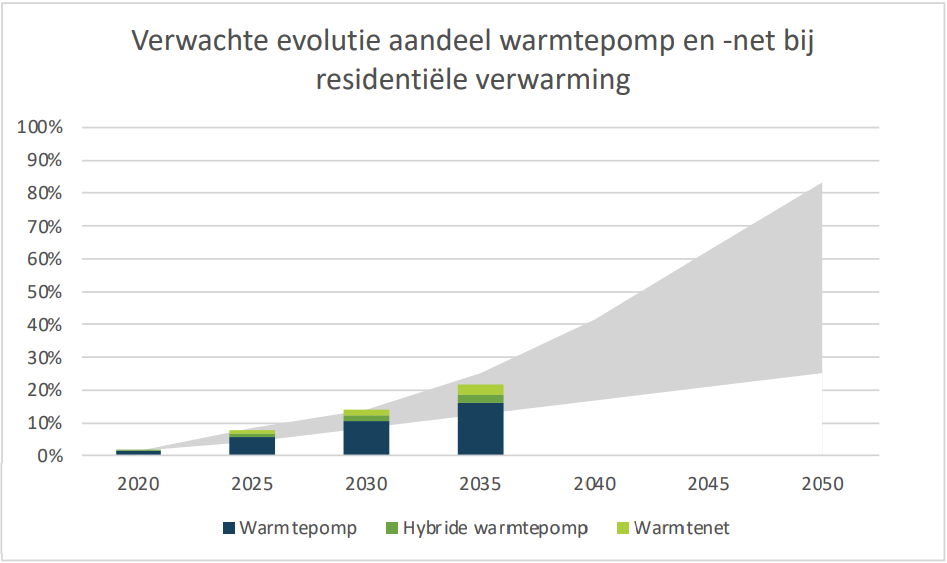
\includegraphics[scale=0.4]{Evolutie_Warmtepomp}
    \caption{\label{fig:Evolutie_Warmtepompen}Verwachte evolutie van het aandeel warmtepomp en -net bij
        residentiële verwarming in Vlaanderen \autocite{Verdoodt2022}.}
\end{figure}

\begin{figure}
    \centering\includegraphics[scale=0.4]{Evolutie_PV}
    \caption{\label{fig:Evolutie_PV}Verwachte evolutie van zonnepanelen in Vlaanderen \autocite{Verdoodt2022}.}
\end{figure}

\begin{figure}
    \centering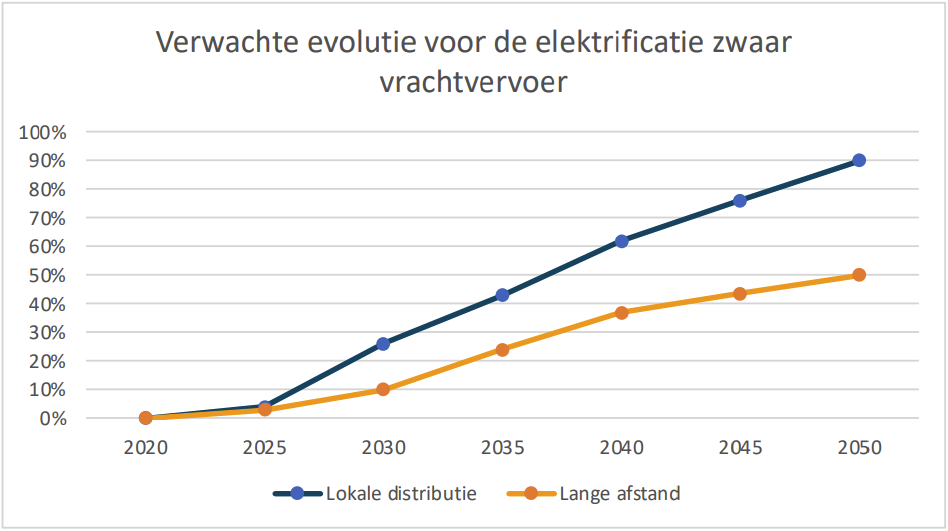
\includegraphics[scale=0.4]{Elektrificatie_Vrachtvervoer}
    \caption{\label{fig:El_Vrachtvervoer}Verwachte evolutie van de elektrificatie van zwaar
        vrachtvervoer in Vlaanderen \autocite{Verdoodt2022}.}
\end{figure}

Om al te hoge investeringen in de distributienetten te vermijden, wordt door Fluvius ingezet op maatregelen die de belasting van het elektriciteitsnet kunnen verminderen en spreiden. Een van die maatregelen is de invoering en verplichting van de digitale elektriciteitsmeter. Tegen juli 2029 moeten alle Belgische huishoudens een digitale meter hebben. Deze digitale meters kunnen via een dongle en een app 'slimmer' gemaakt worden, zodat gezinnen hun elektriciteitsverbruik in detail kunnen opvolgen en bijsturen. Dit zal dan meteen ook een besparing voor hen opleveren. Deze apps vereisen echter steeds een actieve opvolging van de gebruiker. Uit onderzoek is gebleken dat deze actieve bijsturing na verloop van tijd vermindert \autocite{Wemyss2019}. Een enquête van de Vlaamse Regulator van de Elektriciteits- en Gasmarkt \textcite{VREG2021} waarin 1.000 Vlaamse gezinnen en 1.500 bedrijven bevraagd werden over hun ervaring en gedrag op de energiemarkt toont zelfs aan dat van de 60\% van de gezinnen met een digitale meter, slechts 8\% hun energieverbruik effectief bijstuurt. Door de invoering van het capaciteitstarief, een andere maatregel waarmee de VREG het elektriciteitsnet hoopt te ontlasten, zal de bijsturing en vooral spreiding van het elektriciteitsverbruik nog belangrijker worden voor gezinnen. Sinds 1 januari 2023 wordt immers een deel van de nettarieven die een gezin via haar elektriciteitsfactuur betaalt ook berekend op het maximale elektriciteitsverbruik. Er wordt dus voortaan ook gekeken naar de maximale capaciteit die de distributienetbeheerders ter beschikking moeten stellen. Bedoeling van het capaciteitstarief is dat gezinnen hun stroomverbruik beter gaan spreiden. Als iedereen op hetzelfde moment veel stroom verbruikt, kan het net overbelast raken. Het gevolg is dat netbedrijven dan extra moeten investeren in zwaardere elektriciteitskabels om die hogere verbruikspieken op te vangen \autocite{Selleslagh2022}. \\

Daarom wordt binnen Fluvius de vraag gesteld hoe nieuwe technologieën en technieken een oplossing kunnen bieden om gezinnen te helpen bij het spreiden van hun elektriciteitsverbruik. Kunnen apps die het elektriciteitsverbuik monitoren slimmer gemaakt worden zodat ze geen tussenkomst van een gebruiker meer behoeven? Kan bijvoorbeeld artificiële intelligentie (AI) daarbij een oplossing bieden? Om dit na te gaan, zal tijdens dit onderzoek een app ontwikkeld worden die het elektriciteitsverbruik zal aansturen op basis van weersvoorspellingen en historische verbruiksdata.

\section{\IfLanguageName{dutch}{Onderzoeksvraag}{Research question}}%
\label{sec:onderzoeksvraag}

%Wees zo concreet mogelijk bij het formuleren van je onderzoeksvraag. Een onderzoeksvraag is trouwens iets waar nog niemand op dit moment een antwoord heeft (voor zover je kan nagaan). Het opzoeken van bestaande informatie (bv. ``welke tools bestaan er voor deze toepassing?'') is dus geen onderzoeksvraag. Je kan de onderzoeksvraag verder specifiëren in deelvragen. Bv.~als je onderzoek gaat over performantiemetingen, dan 

Kan het elektriciteitsverbruik van gezinnen automatisch bijgestuurd en gespreid worden met behulp van artificiële intelligentie om zo de elektriciteitskost te drukken? \\

Kan een app die het elektriciteitsverbruik en de door zonnepanelen geproduceerde elektriciteit meet en voorspelt ervoor zorgen dat het toekomstige elektriciteitsverbruik beter wordt afgestemd op de zelf geproduceerde stroom?

\section{\IfLanguageName{dutch}{Onderzoeksdoelstelling}{Research objective}}%
\label{sec:onderzoeksdoelstelling}

%Wat is het beoogde resultaat van je bachelorproef? Wat zijn de criteria voor succes? Beschrijf die zo concreet mogelijk. Gaat het bv.\ om een proof-of-concept, een prototype, een verslag met aanbevelingen, een vergelijkende studie, enz.

Om na te gaan of het elektriciteitsverbruik van een gezin automatisch kan gestuurd en gespreid worden, zal een app ontwikkeld worden die in de eerste plaats het elektriciteitsverbruik en de zelf geproduceerde stroom van zonnepanelen inzichtelijk maakt. De gemeten gegevens zullen daarna samen met de weerdata van een weer API gebruikt worden om met artificiële intelligentie een voorspelling van de elektriciteitsproductie en -consumptie te maken. De app zal vervolgens op basis van de gemaakt voorspellingen twee slimme stekkers kunnen aansturen, zodat het elektriciteitsverbruik zo nauwkeurig mogelijk samenvalt met de voorspelde elektriciteitsproductie. 

\section{\IfLanguageName{dutch}{Opzet van deze bachelorproef}{Structure of this bachelor thesis}}%
\label{sec:opzet-bachelorproef}

% Het is gebruikelijk aan het einde van de inleiding een overzicht te
% geven van de opbouw van de rest van de tekst. Deze sectie bevat al een aanzet
% die je kan aanvullen/aanpassen in functie van je eigen tekst.

De rest van deze bachelorproef is als volgt opgebouwd:

In Hoofdstuk~\ref{ch:stand-van-zaken} wordt een overzicht gegeven van de stand van zaken binnen het onderzoeksdomein, op basis van een literatuurstudie.

In Hoofdstuk~\ref{ch:methodologie} wordt de methodologie toegelicht en worden de gebruikte onderzoekstechnieken besproken om een antwoord te kunnen formuleren op de onderzoeksvragen.

% TODO: Vul hier aan voor je eigen hoofstukken, één of twee zinnen per hoofdstuk

In Hoofdstuk~\ref{ch:conclusie}, tenslotte, wordt de conclusie gegeven en een antwoord geformuleerd op de onderzoeksvragen. Daarbij wordt ook een aanzet gegeven voor toekomstig onderzoek binnen dit domein.
\chapter{\IfLanguageName{dutch}{Stand van zaken}{State of the art}}%
\label{ch:stand-van-zaken}

% Tip: Begin elk hoofdstuk met een paragraaf inleiding die beschrijft hoe
% dit hoofdstuk past binnen het geheel van de bachelorproef. Geef in het
% bijzonder aan wat de link is met het vorige en volgende hoofdstuk.

% Pas na deze inleidende paragraaf komt de eerste sectiehoofding.

%Dit hoofdstuk bevat je literatuurstudie. De inhoud gaat verder op de inleiding, maar zal het onderwerp van de bachelorproef *diepgaand* uitspitten. De bedoeling is dat de lezer na lezing van dit hoofdstuk helemaal op de hoogte is van de huidige stand van zaken (state-of-the-art) in het onderzoeksdomein. Iemand die niet vertrouwd is met het onderwerp, weet nu voldoende om de rest van het verhaal te kunnen volgen, zonder dat die er nog andere informatie moet over opzoeken \autocite{Pollefliet2011}.

%Je verwijst bij elke bewering die je doet, vakterm die je introduceert, enz.\ naar je bronnen. In \LaTeX{} kan dat met het commando \texttt{$\backslash${textcite\{\}}} of \texttt{$\backslash${autocite\{\}}}. Als argument van het commando geef je de ``sleutel'' van een ``record'' in een bibliografische databank in het Bib\LaTeX{}-formaat (een tekstbestand). Als je expliciet naar de auteur verwijst in de zin (narratieve referentie), gebruik je \texttt{$\backslash${}textcite\{\}}. Soms is de auteursnaam niet expliciet een onderdeel van de zin, dan gebruik je \texttt{$\backslash${}autocite\{\}} (referentie tussen haakjes). Dit gebruik je bv.~bij een citaat, of om in het bijschrift van een overgenomen afbeelding, broncode, tabel, enz. te verwijzen naar de bron. In de volgende paragraaf een voorbeeld van elk.

%\textcite{Knuth1998} schreef een van de standaardwerken over sorteer- en zoekalgoritmen. Experten zijn het erover eens dat cloud computing een interessante opportuniteit vormen, zowel voor gebruikers als voor dienstverleners op vlak van informatietechnologie~\autocite{Creeger2009}.

%Let er ook op: het \texttt{cite}-commando voor de punt, dus binnen de zin. Je verwijst meteen naar een bron in de eerste zin die erop gebaseerd is, dus niet pas op het einde van een paragraaf. \\

Met een digitale elektriciteitsmeter kunnen gezinnen hun elektriciteitsverbruik makkelijk opvolgen. Dat kan in de eerste plaats gratis via het online energieportaal \href{https://login.fluvius.be/klanten.onmicrosoft.com/b2c_1a_customer_signup_signin/oauth2/v2.0/authorize?client_id=91bb9a0a-f45d-491a-ae0b-43324fbc343a&scope=openid%20profile%20offline_access&redirect_uri=https%3A%2F%2Fmijn.fluvius.be%2Fredirect&client-request-id=90c12c72-7d7b-428b-98fc-5d7956e53a60&response_mode=fragment&response_type=code&x-client-SKU=msal.js.browser&x-client-VER=2.23.0&client_info=1&code_challenge=jz-1E8AwB15UEa352eC_5x6zDtAtwp3Je6jrFVdGKjk&code_challenge_method=S256&nonce=cee3d720-d931-4b13-b0b5-c473169ca6fd&state=eyJpZCI6IjRhM2I3M2NkLTgyZjgtNDFjOC05NzAyLTEwMTNjNjNkNjNhMyIsIm1ldGEiOnsiaW50ZXJhY3Rpb25UeXBlIjoicmVkaXJlY3QifX0%3D}{Mijn Fluvius}. Daarnaast bestaan er ook heel wat gratis of betalende online apps die met een digitale meter kunnen verbonden worden om elektriciteitsverbruik op te volgen en eventueel bij te sturen. Zo’n slimme toepassingen heten in het jargon ‘HEMS’ (Home Energy Management System) of ‘CEMS’ (Customer Energy Management System). De aansluiting van deze apps gebeurt via de gebruikerspoorten (P1 en S1) van de digitale elektriciteitsmeter. Beide gebruikerspoorten zijn complementair en geschikt voor verschillende toepassingen. De P1-poort stuurt de elektriciteitsdata per seconde uit. Via de ‘snelle’ S1-poort worden ruwe data aan een zeer hoge frequentie ter beschikking gesteld aan een app of slimme thermostaat. Dit laat gedetailleerde verbruikersfeedback en sturing toe. Recente digitale elektriciteitsmeters hebben evenwel geen S1-poort meer. De verbinding tussen het meettoestel en een app gebeurt in de meeste gevallen via een wifiverbinding of 4G. Een overzicht van deze toepassingen vindt men op de website \href{https://maakjemeterslim.be/}{www.maakjemeterslim.be}.

\section{\IfLanguageName{dutch}{Overzicht functionaliteiten bestaande apps}{Overview functionalities existing apps}}%
\label{sec:overzicht functionaliteiten bestaande apps}

De bestaande apps bieden allemaal de mogelijkheid om elektriciteitsverbruik in real time op te volgen. Zo kan de gebruiker per dag, per week of per maand nagaan hoeveel elektriciteit er verbruikt en/of geproduceerd werd. Het meten van de energiekosten per huishoudtoestel is ook meestal standaard voorzien, maar geldt even vaak als een optie. De meeste apps sporen ook sluipverbruik op en bieden gepersonaliseerde tips voor energiebesparing. Sommige apps bieden tenslotte ook de mogelijkheid om het gemeten elektriciteitsverbruik naast weerdata te leggen en op die manier na te gaan hoeveel stroom men verbruikt bij bepaalde weersomstandigheden \autocite{Deman2021}. Toen ik vorig jaar mijn onderzoeksvoorstel voor deze bachelorproef formuleerde en uitschreef voor het vak 'Research methods' was er nog geen enkele app die de inzichten in het elektriciteitsverbruik gebruikte om automatisch apparten aan te sturen. Het was toen aan de gebruiker zelf om op basis van de gevevens die de app hem toonde actie te ondernemen en toestellen te gaan in- of uitschakelen. Zoals reeds eerder werd vermeld, leidde dit niet altijd tot de gewenste gedragsverandering \autocite{Wemyss2019}, \autocite{Mack2019} en  \autocite{VREG2021}. Ondertussen zijn een aantal apps daarom uitgebreid met de optie om (huishoud)apparaten automatisch in te schakelen via slimme stekkers. Zes apps voorzien momenteel in de optie om toestellen in te schakelen volgens elektriciteitstarieven of het overschot aan zelf geproduceerde stroom van zonnepanelen, daarbij telkens rekening houdend met het piekverbruik zodat een hoger capaciteitstarief vermeden wordt. Dit gebeurt met bijgeleverde slimme stekkers die via wifi kunnen aangestuurd worden. De automatische aansturing gebeurt echter steeds op het moment zelf, wanneer de app merkt dat er een overschot aan elektricteitsproductie is of de elektriciteitsprijzen laag zijn. Tot op heden is er evenwel nog geen app die gebruik maakt van artificiële intelligentie om de zelf geproduceerde zonne-energie te voorspellen. Dit laat de gebruiker immers toe om de vaatwasser of wasmachine op voorhand  in te laden, zodat de automatische aansturing ervan de volgende dag ook effectief kan gebeuren. 

\section{\IfLanguageName{dutch}{Voorspellingen maken met AI}{Making predictions with AI}}%
\label{sec:voorspellingen maken met AI}

Artificiële intelligentie (AI) verwijst naar de mogelijkheid van applicaties of machines om menselijke vaardigheden te tonen, zoals redeneren, leren en plannen. De term AI wordt vaak gebruikt om andere gerelateerde technieken aan te duiden, zoals machine learning (ML) en deep learning. ML en deeplearning kunnen inderdaad onder de verzamelnaam AI vallen, maar omgekeerd is dit niet altijd het geval. De verschillende technieken van AI hebben immers elk hun eigen doel en opzet. Zo is ML bijvoorbeeld gericht op de studie en de ontwikkeling van algoritmen die kunnen leren of hun prestaties kunnen verbeteren op basis van de data waarmee ze gevoed worden. Machine learning is daarom zeer geschikt om voorspellingen te maken op basis van data uit het verleden. 

\subsection{\IfLanguageName{dutch}{Machine learning}{Machine learning}}%
\label{sec:machine learning}

Machine learning kan opnieuw onderverdeeld worden in drie verschillende categorieën, namelijk supervised learning, unsupervised learning en reinforcement learning. 

\subsubsection{Supervised learning}

Bij supervised machine learning wordt een algoritme door de mens aangeleerd welke conclusies het moet trekken. Er wordt daarbij gewerkt met gelabelde data, wat betekent dat voor elke invoer de gewenste uitvoer bekend is. Het doel van het algoritme is om een model te bouwen dat de relatie tussen invoer en uitvoer begrijpt en deze kan toepassen op nieuwe, ongeziene gegevens. Indien een waarde of getal voorspeld wordt, spreekt men van een regressie. Heeft de voorspelling betrekking op een groep of categorie, dan is er sprake van classificatie \autocite{Brownlee2023}. \\

Een voorbeeld van supervised learning is het voorspellen van huizenprijzen. Een model wordt daarbij getraind op een dataset van huizen waarvan de verkoopprijzen bekend zijn, samen met relevante kenmerken zoals locatie, grootte, aantal slaapkamers, enz. Het model leert vervolgens de relatie tussen deze kenmerken en de verkoopprijs van het huis. Als het model dan een nieuw huis met bijhorende kenmerken herkent, zal het de verkoopprijs ervan kunnen voorspellen.

\subsubsection{Unsupervised learning}

Unsupervised machine learning verloopt op een meer zelfstandige manier. Hierbij leert een algoritme om complexe processen en patronen te identificeren zonder de begeleiding van een mens. Bij unsupervised machine learning vindt training plaats op basis van data die geen labels of een specifieke, vooraf gedefinieerde output hebben  \autocite{Brownlee2023}. \\

Het misschien wel meest gekende voorbeeld van unsupervised learning zijn de aanbevelingen die streamingsplatformen zoals Netflix of Spotify aan hun kijkers aanbieden. Algoritmes analyseren het kijk- en luistergedrag van de gebruikers om daarin patronen en voorkeuren te ontdekken. Vervolgens kunnen dan gepersonaliseerde aanbevelingen gedaan worden.

\subsubsection{Reinforcement learning}

Bij reinforcement leert een algortime of cumputersysteem hoe het moet handelen in een omgeving om een bepaald doel te bereiken. Dit gebeurt door het uitvoeren van acties en het ontvangen van feedback in de vorm van beloningen of straffen. Wat reinforcement learning specifiek maakt is dat het leerproces vergelijkbaar is met hoe een mens of dier zou leren door trial-and-error en beloningen \autocite{Efimov2024}. \\

Reinforcement learning wordt gebruikt in robotica, bijvoorbeeld om robots autonoom te laten navigeren in een omgeving. Om een robot obstakels te leren vermijden wordt gewerkt met beloningen en straffen. Voor elke correcte beweging richting het doel zal de robot een beloning ontvangen. Omgekeerd zal de robot bestraft worden voor elke incorrecte beweging die gemaakt wordt. \\

De applicatie die als proof of concept ontwikkeld wordt voor deze bachelorproef, zal de toekomstige stroomproductie van zonnepanelen gaan voorspellen. Hiervoor zullen historische zonnestralingsgegevens gebruikt worden. Er zal dus gebruik gemaakt worden van de supervised learning methode en meer specifiek zal het regressiemodel toegepast worden. De waarde die moet voorspeld worden is de hoeveelheid zonnestraling uitgedrukt in Watt/m².

\subsection{\IfLanguageName{dutch}{Supervised machine learning: regressie modellen}{Supervised machine learning: regression models}}%
\label{sec:supervised machine learning: regressie modellen}

\subsubsection{Decision Tree Regression (DTR)}

Het Decision Tree model is een regressiealgoritme dat een dataset systematisch opdeelt in steeds kleinere homogene subgroepen op basis van de kenmerken van de gebruikte dataset. Het ontwikkelt daarbij een beslissingsboom, waarbij de interne knooppunten de kenmerken van de dataset vertegenwoordigen, de takken de beslissingsregles en elke bladknoop het resultaat. In de beslissingsboom zijn er twee knooppunten, namelijk de beslissingsknooppunten en de bladknooppunten. Beslissingsknooppunten worden gebruikt om een beslissing te nemen en hebben meerdere takken, terwijl Bladknooppunten de uitkomst van die beslissingen zijn en geen verdere takken bevatten.
De beslissingen of de test worden uitgevoerd op basis van de kenmerken van de gegeven dataset. Het doel is om eenvoudige beslissingsregels te leren op basis van die specifieke kenmerken van de dataset om zo een model te ontwikkelen dat een bepaalde waarde voorspelt  \autocite{Balakumar2023}.  
\\
\begin{figure}[h!]
    \centering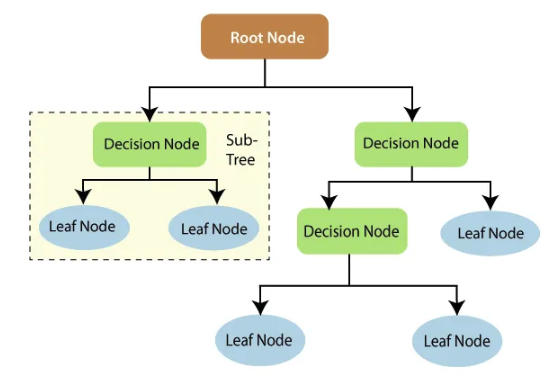
\includegraphics[scale=0.55]{Decision_Tree }
    \caption{\label{fig:Decision_Tree}Grafische voorstelling beslissingsboom.}
\end{figure} 
\\

Decision trees zijn makkelijk te interpreteren omdat de geleerde beslissingsregels makkelijk te begrijpen en visualiseren zijn. Bovendien kan het DTR-algoritme niet-lineaire en dus meer complexe relaties tussen de inputvariabelen en de voorspelde waarde ontdekken, wat het algoritme zeer bruikbaar maakt voor datasets die complexe patronen bevatten  \autocite{Viswa2023}. 

\subsubsection{Random Forest Regression (RFR)}

Het Random Forest regressie model bestaat uit een verzameling van zogenaamde decision trees of beslissingsbomen. Een beslissingsboom is op zijn beurt een schema dat is opgebouwd uit een opeenvolging van binaire beslissingsregels. Het is een grafische voorstelling van een probleemstelling waarin verschillende mogelijke alternatieven met gebeurtenissen worden weergegeven en uitgewerkt. Het RFR-model maakt meerdere beslissingbomen aan op basis van willekeurig gekozen subsets van de gebruikte dataset. Het model voegt vervolgens de uitkomsten van al deze beslissingbomen samen om een algemene voorspelling te doen voor ongekende datapunten. Daarbij wordt telkens het gemiddelde of gewogen gemiddelde van elke beslissingsboom genomen. Op deze manier kan het grotere datasets verwerken en complexere verbanden vastleggen dan individuele beslissingsbomen. Het geheel van de voorspellingen van de beslissingbomen zorgt voor een grotere accuraatheid dan de voorspelling van één enkele beslissingsboom. Over het algemeen kan gesteld worden dat hoe meer beslissingsbomen er in het RFR-model zitten, des te robuster het model zal zijn \autocite{Balakumar2023}. \\

\begin{figure}[h!]
    \centering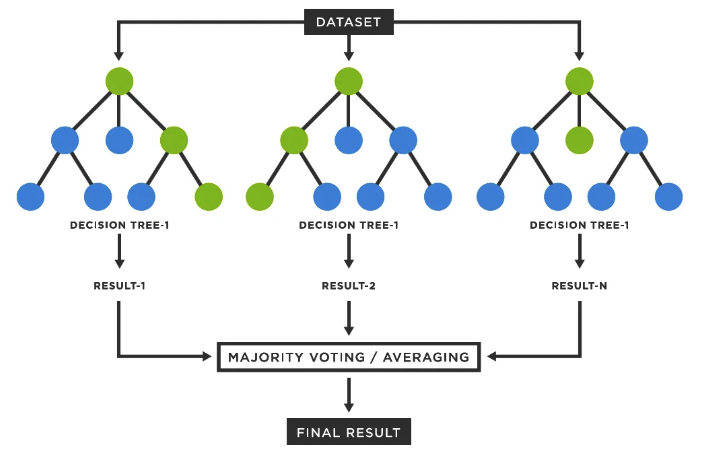
\includegraphics[scale=0.5]{Random_Forest}
    \caption{\label{fig:Random_Forest}Grafische voorstellingvan het Random Forest algoritme.}
\end{figure} 

Het RFR-model wordt vaak gebruikt om continue waarden te voorspellen, zoals aandelenkoersen, tijdreeksen of verkoopprijzen. Het is minder gevoelig voor 'overfitting' (dit doet zich voor wanneer een ML-model de trainingsdata te goed leert, waardoor het nieuwe ongekende data slecht voorspelt) dan andere regressiemethoden omdat het meerdere willekeurige bomen onafhankelijk van elkaar opbouwt en een gemiddelde van de individuele voorspellingen neemt. Het is een goede keuze wanneer data gebruikt wordt met veel verschillende kenmerken of inputvariabelen  \autocite{Sahai2023}.

\subsubsection{Support Vector Machine (SVM)}

Het Support Vector Machine algoritme probeert data zo optimaal mogelijk in twee groepen te verdelen door het vinden van het beste hyperplane. Deze hyperplane is de meest optimale scheidingslijn tussen de twee groepen van data. Het algoritme maakt daarbij gebruik van support vectors. Dit zijn de datapunten die zich het dichtst bij de optimale scheidingslijn bevinden. Om de meest optimale scheidingslijn te achterhalen, berekent het algoritme de maximale marge of afstand tussen de datapunten van de twee groepen  \autocite{Tziolis2024}. Omdat het algoritme zeer effectief is in het oplossen van complexere, niet-lineaire problemen, is het een model dat vaak grbuikt wordt om voorspellingen te maken op het gebied van hernieuwbare energie \autocite{Ahmad2018}. \\

\begin{figure}[h!]
    \centering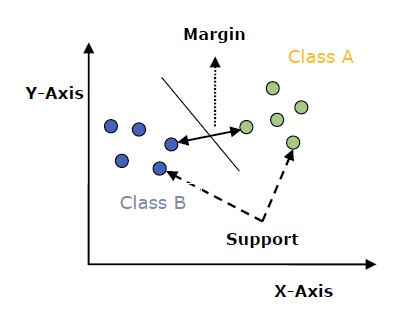
\includegraphics[scale=0.7]{SVM}
    \caption{\label{fig:SVM}Grafische voorstelling Support Vector Machine.}
\end{figure} 

Het SVM-model wordt typisch gebruikt voor kleinere datasets omdat de trainigstijd van dit algoritme zeer lang kan zijn. Het wordt ook vooral toegepast op 'proper' datasets, dit zijn datasets die weinig afwijkingen of fouten bevatten.

\subsubsection{Autoregressive Integrated Moving Average (ARIMA)}

Het Autoregressive Integrated Moving Average (ARIMA) model is een populair voorspellingsmodel voor tijdreeksen. Het wordt veel gebruikt op verschillende gebieden om toekomstige waarden te analyseren en te voorspellen op basis van waarnemingen uit het verleden in een tijdreeksdataset. \\

Het ARIMA-model combineert drie belangrijke componenten: Autoregressie (AR), differentiëren (I) en voortschrijdend gemiddelde (MA). \\

AR - Autoregressief (p): Dit verwijst naar de afhankelijkheid van de huidige waarde in een tijdreeks van eerdere waarden. De volgorde van de AR-component, aangeduid met p, vertegenwoordigt het aantal vertraagde waarnemingen die in het model worden gebruikt. \\

I - Integratievolgorde (d): Dit is het aantal verschillen dat we beschouwen tussen de huidige waarde en de waarde in het verleden om de tijdreeks stationair te maken. Stationair betekent dat de statistische eigenschappen van de reeks, zoals gemiddelde en variantie, constant blijven in de tijd. \\

MA - Bewegend gemiddelde (q): Het vertegenwoordigt de afhankelijkheid tussen de huidige waarde en de restfouten van voorspellingen uit het verleden. Het berekent het gewogen gemiddelde van de vorige voorspellingsfouten. De volgorde van de MA-component, aangeduid met q, geeft het aantal vertraagde voorspellingsfouten weer die in het model worden gebruikt.

\subsubsection{Long Short-Term Memory (LSTM)}

Het Long Short-Term Memory (LSTM) is een type Recurrent Neural Network (RNN) dat wordt gebruikt om temporele afhankelijkheden in gegevens te modelleren. Concreet kan het zich gebeurtenissen uit het verleden of afhankelijkheden uit eerder waargenomen periodes herinneren. \\

Een LSTM is een type netwerk dat speciaal is ontworpen om een computer te helpen informatie langer te onthouden dan gewoonlijk mogelijk is met een terugkerend neuraal netwerk. Het lange-kortetermijngeheugenmodel werkt met behulp van ‘cellen’ die informatie gedurende langere tijd opslaan; wanneer een nieuwe invoer wordt gedetecteerd, worden er nieuwe cellen gemaakt die aan de bestaande cellen worden gekoppeld. Daarnaast kunnen de nieuwe cellen een deel van de informatie die in de bestaande cellen is opgeslagen ‘vergeten’, waardoor het netwerk een deel van wat het heeft geleerd kan ‘vergeten’. \\

\begin{figure}[h!]
    \centering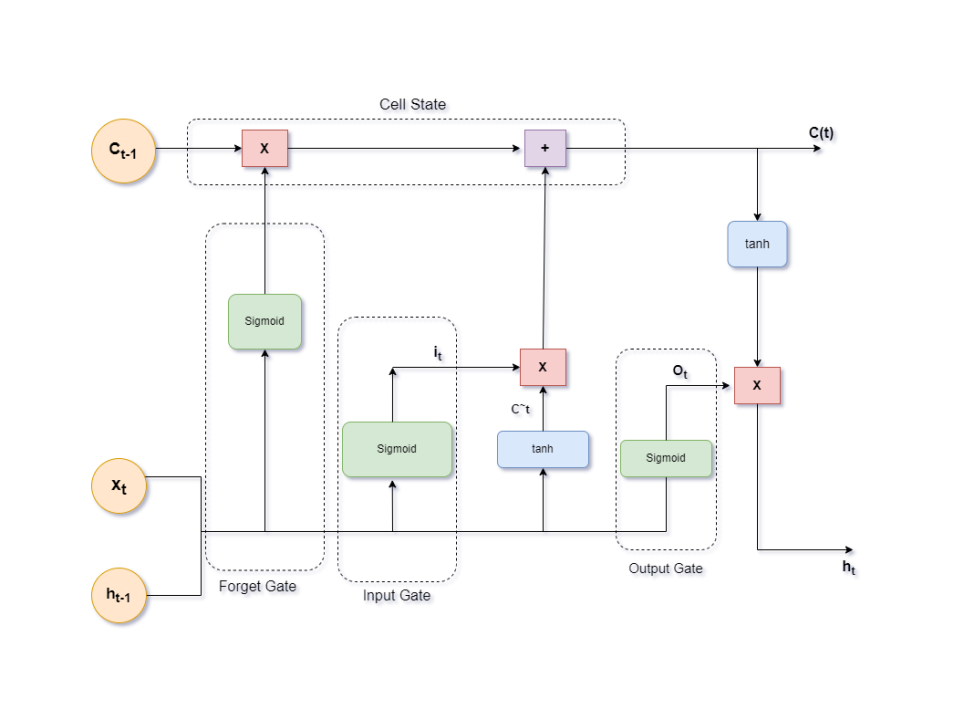
\includegraphics[scale=0.5]{LSTM}
    \caption{\label{fig:LSTM}Grafische voorstellingvan het LSTM algoritme.}
\end{figure} 

De belangrijkste componenten van de LSTM zijn de geheugencellen, vergeetpoorten en invoerpoorten. Geheugencellen zijn verantwoordelijk voor het langdurig opslaan van informatie, en de vergeet- en invoerpoorten beslissen welke informatie wel of niet in de cellen moet worden opgeslagen. Deze componenten zorgen ervoor dat LSTM-netwerken het verleden kunnen ‘herinneren’ en tegelijkertijd rekening kunnen houden met nieuwe input. \\

LSTM's zijn zeer effectief vanwege hun vermogen om informatie gedurende langere tijd op te slaan en nieuwe input efficiënter te verwerken dan traditionele terugkerende neurale netwerken.

\subsubsection{Extreme gradient Boosting (XGBoost)}

Het XGBoost algoritme is een ensemble-leermethode die gradiëntversterking en beslissingsbomen combineert. Het concept van gradiëntversterking verwijst naar het opeenvolgend toevoegen van beslissingsbomen aan het model, waarbij elke volgende boom de fouten corrigeert die door de vorige zijn gemaakt. Dankzij dit iteratieve proces kan het XGBoost zijn voorspellingen voortdurend verbeteren en een hoge nauwkeurigheid bereiken.De werking van beslissingsbomen is hierboven reeds toegelicht. \\

\begin{figure}[h!]
    \centering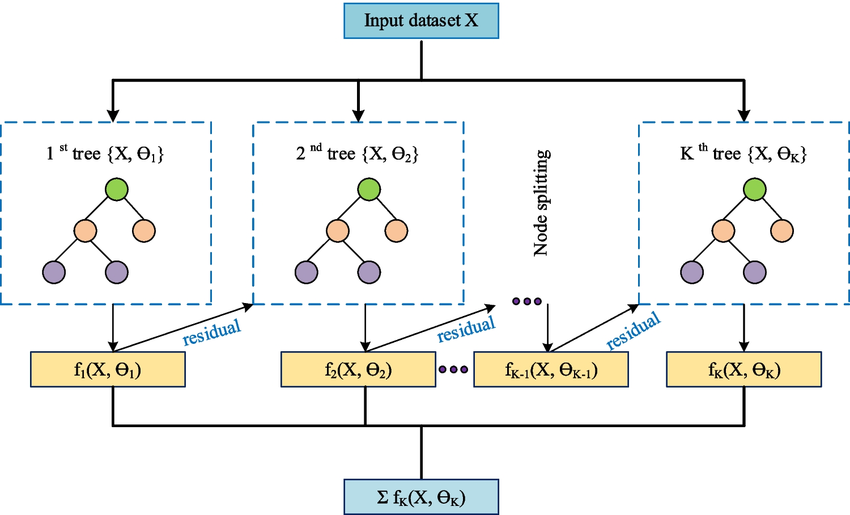
\includegraphics[scale=1.9]{XGBoost}
    \caption{\label{fig:XGBoost}Grafische voorstelling van de structuur van het XGBoost algoritme.}
\end{figure} 

Het XGBoost-model is specifiek ontworpen om de eigen prestaties te optimaliseren en grootschalige datasets efficiënt te verwerken. Door iteratief zwakke voorspellingen toe te voegen, kan het XGBoost algoritme snelle en accurate voorspellingen maken. Het grote voordeel van XGBoost is dat het ingebouwde mechanismen heeft om ontbrekende waarden in de dataset te verwerken. Het kan tijdens het trainingsproces automatisch leren hoe er het beste met ontbrekende waarden kan worden omgegaan. Vermits de meeste datasets uit de echte wereld gegevens ontbreken, is het XGBoost algoritme dus zeer geschikt om voorspellingen te maken. Nog een voordeel van het XGBoost-model is dat het makkelijk schaalbaar is, omdat het gebruik maakt van parallelle verwerkingstechnieken waarbij de werklast over meerdere cores of machines verdeeld wordt. Dit maakt snellere trainings- en voorspellingstijden mogelijk. Deze schaalbaarheid maakt XGBoost geschikt voor toepassingen die realtime voorspellingen vereisen.

\subsection{\IfLanguageName{dutch}{Machine learning modellen evalueren}{Evaluate machine learning models}}%
\label{sec:Machine learning modellen evalueren}

Er bestaan verschillende methodes waarmee de kwaliteit en nauwkeurigheid van een machine learning model kan gemeten worden. De meest gebruikte zijn:

\subsubsection{Mean absolute error (MAE)}

De Mean Absolute Error (MAE) of gemiddelde absolute fout is het gemiddelde van alle absolute voorspellingsfouten waarbij de voorspellingsfout het verschil is tussen de werkelijke en de voorspelde waarde. Het wordt berekend door de absolute verschillen tussen voorspelde waarden en werkelijke waarden bij elkaar op te tellen en te delen door het aantal waarnemingen. Door de absolute waarde van voorspellingsfouten te gebruiken wordt voorkomen dat positieve en negatieve fouten elkaar opheffen. Hoe kleiner de waarde van de MAE, des te beter de voorspellingen van een model overeenstemmen met de werkelijke waarden.

\subsubsection{Mean Squared Error (MSE)}

Mean Squared Error (MSE) of gemiddelde kwadratische fout is de gemiddelde kwadratische afwijking tussen de voorspelde waarden van een model en de werkelijke waarden. Een lagere MSE geeft aan dat de voorspellingen van een model dichter bij de werkelijkheid liggen en het model dus nauwkeuriger is.

\subsubsection{Root mean squared error (RMSE)}

Root Mean Squared Error (RMSE) of vierkantswortel van de gemiddelde kwadratische fout is de gemiddelde omvang van de positieve of negatieve verschillen tussen de waarden die door een model voorspeld zijn en de geobserveerde (feitelijke) waarden. Het kan beschouwd worden als de standaardafwijking van de voorspellingsfouten. \\

RMSE biedt één enkele waarde die de prestaties van een model vertegenwoordigt, waardoor een eenvoudige vergelijking tussen verschillende modellen of voorspellingstechnieken mogelijk is. Lagere RMSE-waarden duiden op betere modelprestaties. Een lagere RMSE geeft aan dat de voorspellingen van het model dichter bij de werkelijke waarden liggen, wat een hogere nauwkeurigheid suggereert.

\subsubsection{R-squared (R²)}

De R-squared (R²) of determinatiecoëfficiënt meet in hoeverre een model in staat is een bepaalde uitkomst te voorspellen. Het geeft aan hoe sterk het verband is tussen de werkelijke waarden en de voorspelde waarden van een model. R² is dan ook nauw verwant aan de correlatiecoëfficiënt. Het kwadraat van de correlatiecoëfficiënt tussen de onafhankelijke en afhankelijke variabelen is gelijk aan de R-kwadraatwaarde. Dit impliceert dat een hogere correlatie overeenkomt met een hogere R-kwadraatwaarde. \\

De laagst mogelijke waarde van R² is 0 en de hoogst mogelijke waarde is 1. Hoe beter een model is in het maken van voorspellingen, hoe dichter de determinatiecoëfficiënt R² bij het getal 1 zal liggen.

\section{\IfLanguageName{dutch}{Elektriciteitsproductie voorspellen}{Predict electricity production}}%
\label{sec:elektriciteitsproductie voorspellen}

Doordat het belang van hernieuwbare energie de laatste jaren enorm is toegenomen, is er al heel wat onderzoek verricht naar het voorspellen van de toekomstige stroomproductie van zonnepanelen met behulp van machine learning. In de meeste van deze onderzoeken wordt deze voorspelling gebaseerd op de voorspelling van de hoeveelheid zonnestraling. Een andere optie bestaat erin om de historische stroomproductie van de zonnepanelen te gaan analyseren en daaruit een voorspelling te gaan maken \autocite{Wang2022}. Deze historische stroomproductie data is evenwel niet altijd voldoende voorhanden, zodat het soms niet mogelijk is om op bais daarvan voorspellingen te gaan doen.

\subsection{Zonnestraling}

Vermits zonnepanelen zonne-energie omzetten in elektricteit, is het bijna een logische keuze om de toekomstige stroomproductie van zonnepanelen te gaan voorspellen op basis van de voorspelling van de hoeveelheid zonnestraling \autocite{Ledmaoui2023}. Meestal wordt daarbij de inkomende of globale horizontale instraling (GHI, Global Horizontal Irradiance) voorspeld . GHI is de totale hoeveelheid zonnestraling die het aardoppervlak bereikt en wordt uitgedrukt in W/m². De GHI bestaat uit directe normale instraling (DNI, Direct Normal Irradiance)  en de diffuse horizontale instraling (DHI, Diffuse Horizontal Irradiance). DNI verwijst naar de grootste directe (90 graden) neerwaartse zonnestraling voor een bepaalde plaats. Deze directe normale instraling wordt gebruikt om de diffuse horizontale instraling te berekenen. De DHI is de zonnestraling die niet rechstreeks van de zon komt, maar verspreid is door de wolken en deeltjes in de atmosfeer. Deze zonnestraling komt in gelijke mate uit alle richtingen \autocite{Sehrawat2023}. \\

Historische data met betrekking tot zonnestraling kan vrij verkregen worden via de CAMS Radiation Service (CRS) van de Copernicus Atmosphere Monitoring Service (\href{https://atmosphere.copernicus.eu}{CAMS}). Dit maakt deel uit van het European Earth observation programme Copernicus (EEC) dat informatiediensten biedt op basis van aardobservatiegegevens van satellieten en in-situgegevens (niet uit de ruimte). Enorme hoeveelheden wereldwijde gegevens van satellieten en van meetsystemen op de grond, in de lucht en op zee worden gebruikt om informatie te verstrekken aan dienstverleners, overheidsinstanties, andere internationale organisaties en burgers. De aangeboden informatiediensten zijn gratis en open toegankelijk voor de gebruikers ervan. De geografische dekking van de gegevens is het gebied dat door de Meteosat (een serie geosynchrone weersatellieten van de Europese ruimtevaartorganisaties ESA en EUMETSAT) kan worden waargenomen. Dit gebeid omvat Europa, Afrika en het Midden-Oosten.

\subsection{Meteorologische data}

De hoeveelheid stroom die zonnepanelen produceren is niet enkel afhankelijk van de hoeveelheid zonnestraling. Ook andere meteorologische gegevens spelen hierbij een rol. Zo zijn de temperatuur, de relatieve luchtvochtigheid en de bewolkingsgraad factoren die het meeste invloed hebben op de stroomproductie van zonnepanelen \autocite{Sehrawat2023}. \\

Er zijn verschillende kanalen waarlangs historische weerdata kan verkregen worden. Zo zijn er datasets van meteorologische gegevens die door het Koninklijk Meteorologisch Insituuut (KMI) beschikbaar gesteld worden. Het aantal datasets is echter zeer beperkt en moeten handmatig gedownload worden. Ook via het CAMS kan historische weerdata opgevraagd worden, maar ook deze data is beperkt aangezien de meest recente weerdata van het jaar 2016 is. \\

Er bestaan tal van open source en dus gratis weer API's die makkelijk geïntegreerd kunnen worden met een app. Deze API's bieden voorspellingen aan van verschillend meteorologische gegevens, maar leveren vaak beperkte historische weerdata aan. Voor de historische weerdata werd \href{https://dev.meteostat.net/}{Meteostat} gekozen. Deze open-source API biedt een Pyhon library waarmee met slechts een enkele HTTP-request historische weerdata voor een bepaalde locatie kan worden opgevraagd. Meteostat verzamelt historische weer- en klimaatdata van weerstations en verschillende nationale meteorologische instituten van over de hele wereld. De historische weerdata zal voor dezelfde periode als de zonnestralingsdata opgevraagd worden en op die manier de zonnestralingsdata verrijken, zodat de voorspelling van de toekomstige zonnestaling en stroomproductie van de zonnepanelen accurater wordt. \\

De voorspelling van de toekomstige elektriciteitsproductie van de zonnepanelen zal tenslotte nog proberen verbeterd worden door de voorspelde hoeveelheid zonnestraling te combineren met de weersvoorspellingen voor periode die voorspeld wordt. Omdat Meteostat enkel historische weerdata aanbiedt, werd voor de weersvoorspellingen een andere open-source weer-API gebruikt. \href{https://open-meteo.com/}{Open-Meteo API} werkt ook samen met verschillende nationale meteorologische diensten en biedt betrouwbare weersvoorspellingen aan tot 16 dagen in de toekomst. De aangeboden API-request kan makkelijk aangepast worden, zodat enkel de benodigde weerdata kan worden opgevraagd, wat een gunstig effect heeft op de performantie bij het opvragen van de data.

%%=============================================================================
%% Methodologie
%%=============================================================================

\chapter{\IfLanguageName{dutch}{Methodologie}{Methodology}}%
\label{ch:methodologie}

%% TODO: In dit hoofstuk geef je een korte toelichting over hoe je te werk bent
%% gegaan. Verdeel je onderzoek in grote fasen, en licht in elke fase toe wat
%% de doelstelling was, welke deliverables daar uit gekomen zijn, en welke
%% onderzoeksmethoden je daarbij toegepast hebt. Verantwoord waarom je
%% op deze manier te werk gegaan bent.
%% 
%% Voorbeelden van zulke fasen zijn: literatuurstudie, opstellen van een
%% requirements-analyse, opstellen long-list (bij vergelijkende studie),
%% selectie van geschikte tools (bij vergelijkende studie, "short-list"),
%% opzetten testopstelling/PoC, uitvoeren testen en verzamelen
%% van resultaten, analyse van resultaten, ...
%%
%% !!!!! LET OP !!!!!
%%
%% Het is uitdrukkelijk NIET de bedoeling dat je het grootste deel van de corpus
%% van je bachelorproef in dit hoofstuk verwerkt! Dit hoofdstuk is eerder een
%% kort overzicht van je plan van aanpak.
%%
%% Maak voor elke fase (behalve het literatuuronderzoek) een NIEUW HOOFDSTUK aan
%% en geef het een gepaste titel.

Het onderzoek van deze bachelorproef bestaat uit twee delen. In het eerste deel wordt een literatuurstudie gemaakt om de huidige stand van zaken met betrekking tot het onderwerp van deze bachelorproef inzichtelijk te maken. Er wordt gestart met een overzicht van de functionaliteiten en tekortkomingen van de apps die er momenteel bestaan om een digitale elektriciteitsmeter slimmer te maken. Daarna wordt toegelicht hoe met behulp van AI en meer specifiek machine learning (ML) voorspellingen kunnen gemaakt worden. Er wordt daarbij kort ingegaan op de ML algoritmes die het vaakst gebruikt worden om zonnestraling en stroomproductie van zonnepanelen te voorspellen en hoe de prestaties van deze algoritmes kunnen beoordeeld worden. Vervolgens wordt een overzicht gegeven van de onderzoeken die reeds gevoerd zijn naar de voorspelling van zonnestraling en/of stroomproductie van zonnepanelen met behulp van machine learning. Daarbij wordt ook uitgelegd welke data hiervoor zal gebruikt worden in deze bachelorproef. De literatuurstudie wordt afgesloten met een toelichting over de aansturing van slimme apparaten en de problematiek van het ontbreken van een gestandardiseerd protocol hiervoor. \\

In het tweede deel van deze bachelorproef wordt de ontwikkeling van een proof of concept beschreven.



%%=============================================================================
%% Proof of concept
%%=============================================================================

\chapter{\IfLanguageName{dutch}{Proof of Concept}{Proof of Concept}}%
\label{ch:proofofconcept}

% TODO: Trek een duidelijke conclusie, in de vorm van een antwoord op de
% onderzoeksvra(a)g(en). Wat was jouw bijdrage aan het onderzoeksdomein en
% hoe biedt dit meerwaarde aan het vakgebied/doelgroep? 
% Reflecteer kritisch over het resultaat. In Engelse teksten wordt deze sectie
% ``Discussion'' genoemd. Had je deze uitkomst verwacht? Zijn er zaken die nog
% niet duidelijk zijn?
% Heeft het onderzoek geleid tot nieuwe vragen die uitnodigen tot verder 
%onderzoek?

\section{\IfLanguageName{dutch}{Ontwikkeling van de mobiele app}{Development mobile app}}%
\label{sec:ontwikkeling mobiele app}

Om de onderzoeksvraag van deze bachelorproef te kunnen beantwoorden werden een Python web server en een  iOS app ontwikkeld als proof of concept. Deze app maakt in de eerste plaats het elektriciteitsverbruik en de stroomproductie van de zonnepanelen inzichtelijk. Daarnaast zal de app via de toepassing van machine learning de elektriciteitsproductie van de volgende dag voorspellen. Deze voorspelling zal dan door de app gebruikt worden om de inschakeling van twee slimme stekkers te programmeren indien er voldoende stroomproductie voorspeld wordt.

\subsection{\IfLanguageName{dutch}{Digitale elektriciteitsmeter uitlezen}{Reading out digital electricitymeter}}%
\label{sec:Digitale elektriciteitsmeter uitlezen}

Een mobiele app die het elektriciteitsverbruik wil bijsturen en beter spreiden zal de gebruiker ervan allereerst inzicht moeten geven in zijn of haar verbruik. Om de verbruiksgegevens te ontsluiten moet de digitale elektriciteitsmeter uitgelezen worden via de P1-poort. Hiervoor zijn verschillende mogelijkheden, van een dongle tot kleine toestellen die via een kabel met de P1-poort kunnen verbonden worden. Voor dit onderzoek is er gekozen voor een Raspberry Pi 5 minicomputer om de digitale meter uit te lezen. Deze singleboardcomputer die gebaseerd is op een ARM processor en de Linuxdistributie Ubuntu als besturingssysteem heeft, biedt meer mogelijkheden dan enkel het uitlezen van data. Omdat het verbruik ervan zeer laag is, kan dit toestel bovendien continu ingeschakeld blijven. Daarnaast heeft de Raspberry Pi wifi-ondersteuning, zodat deze kan verbonden worden met het wifinetwerk van de woning die als testomgeving gebruikt wordt. Dit maakt het mogelijk om een webserver op te zetten en meteen ook de omvormer van de zonnepanelen van de woning via het wifinetwerk uit te lezen met de Raspberry Pi (zie volgende sectie). In de testwoning bevindt de digitale elektriciteitsmeter zich namelijk in de kelder, terwijl de omvormer van de zonnepanelen zich op zolder bevindt. Een situatie die wel vaker voorkomt en op deze manier kan worden opgelost.

\begin{figure}[h!]
    \centering
    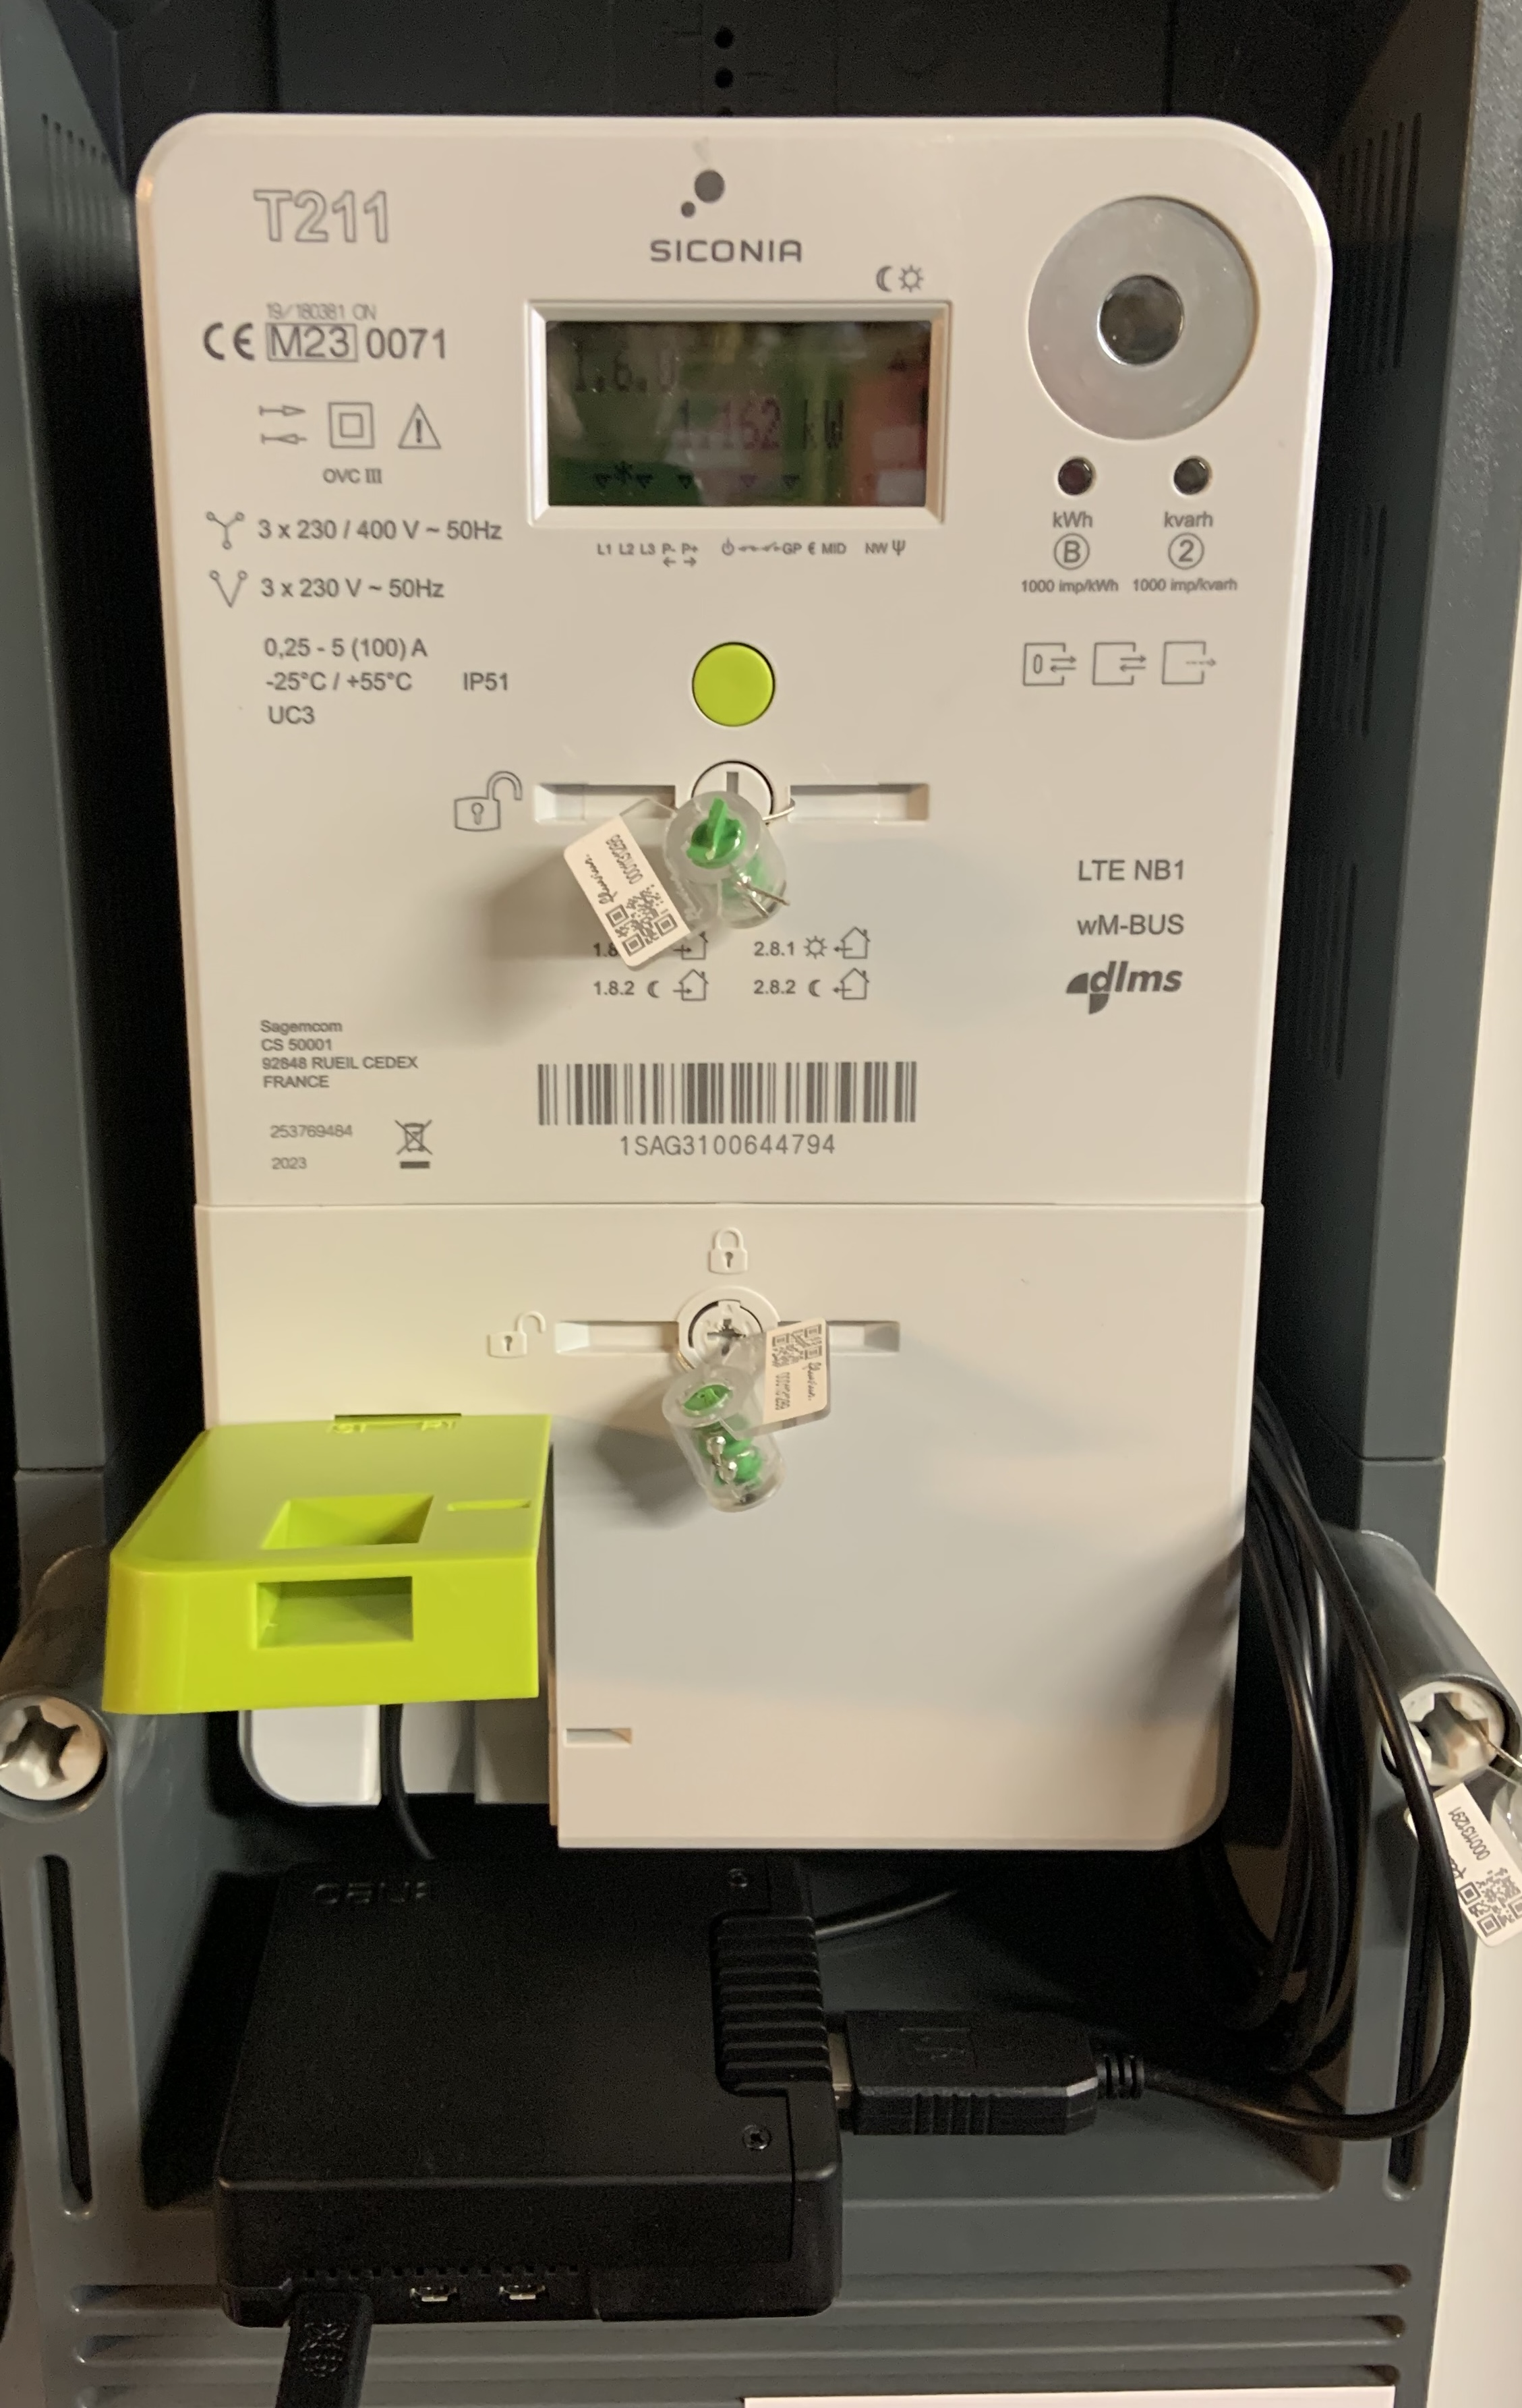
\includegraphics[width=7cm]{TestSetup} \hspace{0.7cm}
    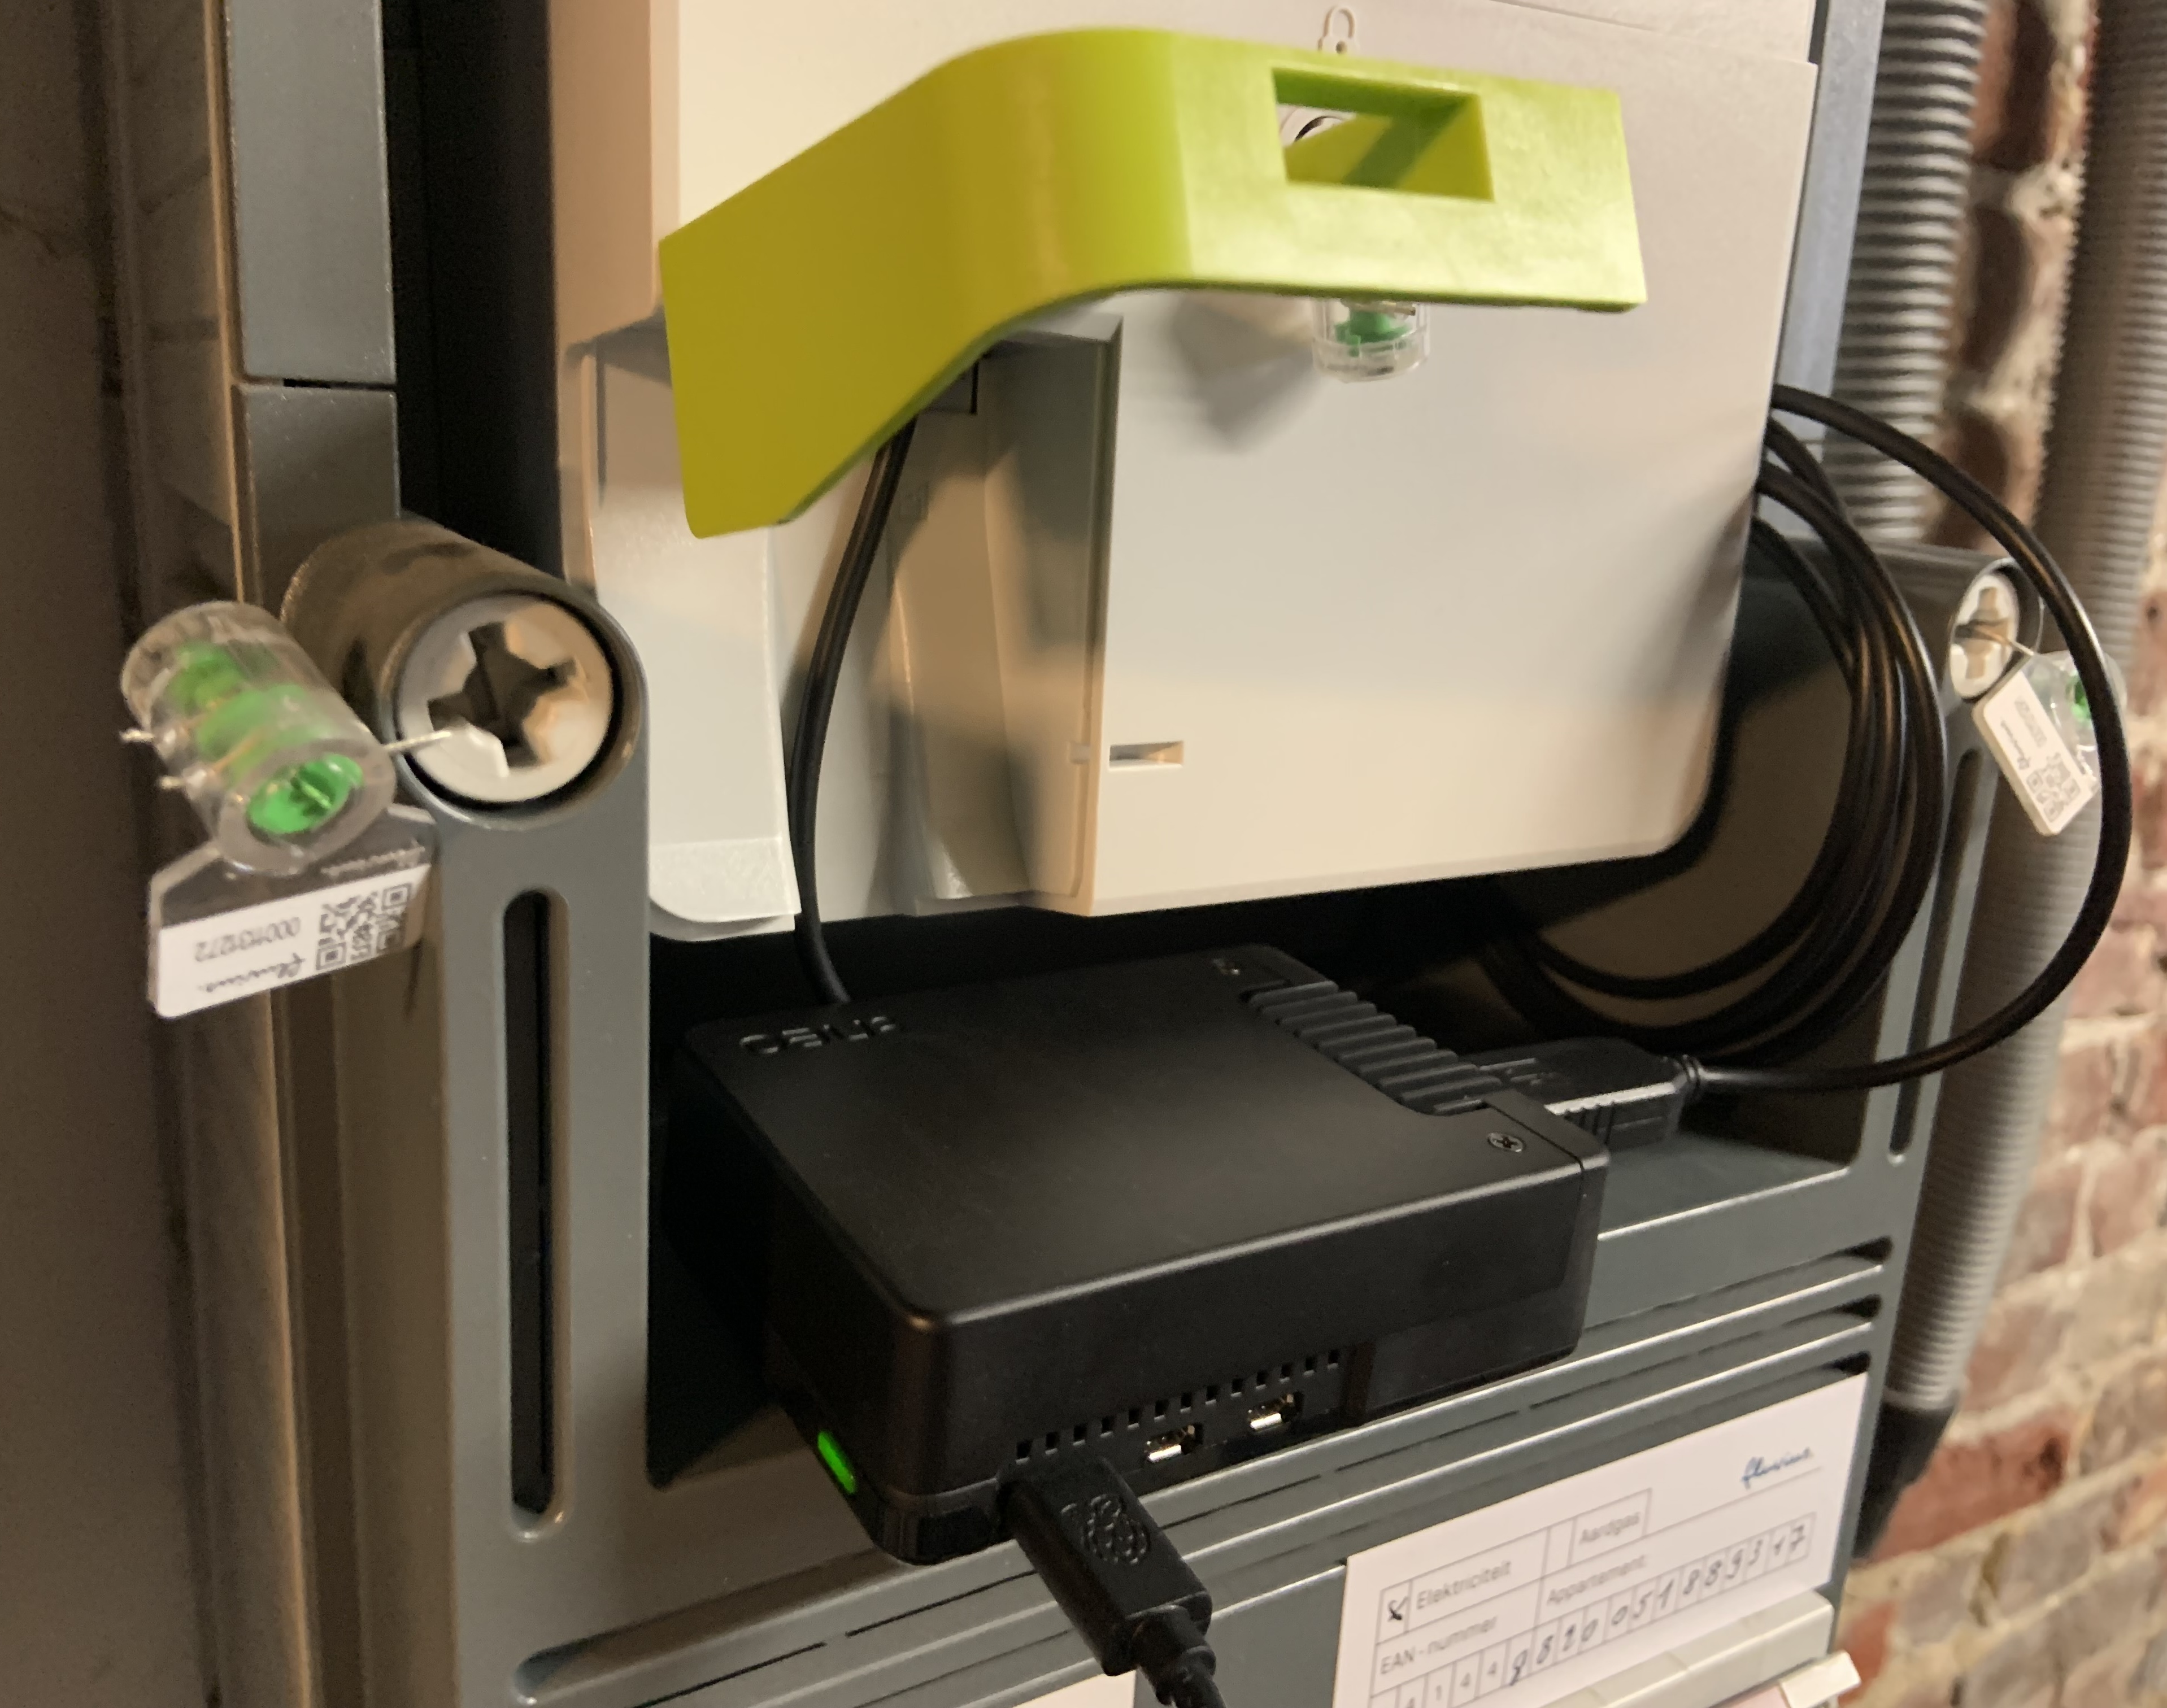
\includegraphics[width=7cm]{RPi5}
    \caption{Testopstelling: Raspberry Pi 5 via een RS422 serieel naar USB kabel aangesloten op een digitale elektriciteitsmeter.}
\end{figure}

\subsubsection{Opslag uitgelezen elektriciteitsdata}

Nadat de Raspberry Pi via de juiste kabel op de P1-poort werd aangesloten, kon de data van de digitale elektriciteitsmeter via een Python script worden uitgelezen. Hiervoor werd een bestaand Python script uitgebreid \autocite{Depuydt2021}. Het bestaande script voorzag enkel in het uitprinten van de uitgelezen data in de console. Om de uitgelezen elektriciteitsdata later via een app te kunnen weergeven moest deze data worden weggeschreven naar een databank. Omdat de data via de P1-poort per seconde uitgelezen wordt, werd geopteerd voor InfluxDB. Deze NoSQL-databank is speciaal ontwikkeld voor tijdreeksen (time series) en is binnen bepaalde (ruime) grenzen gratis te gebruiken \autocite{Balis2017} en  \autocite{Struckov2019}. Het Python script werd tenslotte opgezet als een achtergrond service via de systeem manager voor Linux 'systemctl/systemd', zodat het voortdurend blijft uitgevoerd worden.

\subsection{\IfLanguageName{dutch}{Omvormer zonnepanelen uitlezen}{Reading out power converter PV system}}%
\label{sec:Omvormer zonnepanelen uitlezen}

Zoals reeds vermeld bevindt de omvormer van de zonnepanelen zich op de zolderverdieping, terwijl de Raspberry Pi zich in de kelder bij de digitale elektriciteitsmeter bevindt. De enige mogelijkheid om een draadloze verbinding te maken tussen beide toestellen is via het lokale wifinetwerk. De omvormer in casu heeft echter geen ingebouwde wifi-ondersteuning en diende uitgebreid te worden met een aparte wifistick. Via deze wifistick kon dan vervolgens de data van de omvormer uitgelezen worden. Dit gebeurt opnieuw via een Python script waarin een request wordt gestuurd naar de server van de producent waar de gegevens van de omvormer worden bijgehouden. Omdat de data van de digitale elektriciteitsmeter per seconde wordt uitgelezen, wordt ook de data van de omvormer per seconde opgevraagd. De ontvangen gegevens zijn de temperatuur, de huidige geproduceerde stroom en de totale dagproductie van de zonnepanelen. \\

\begin{figure}[h!]
    \centering
    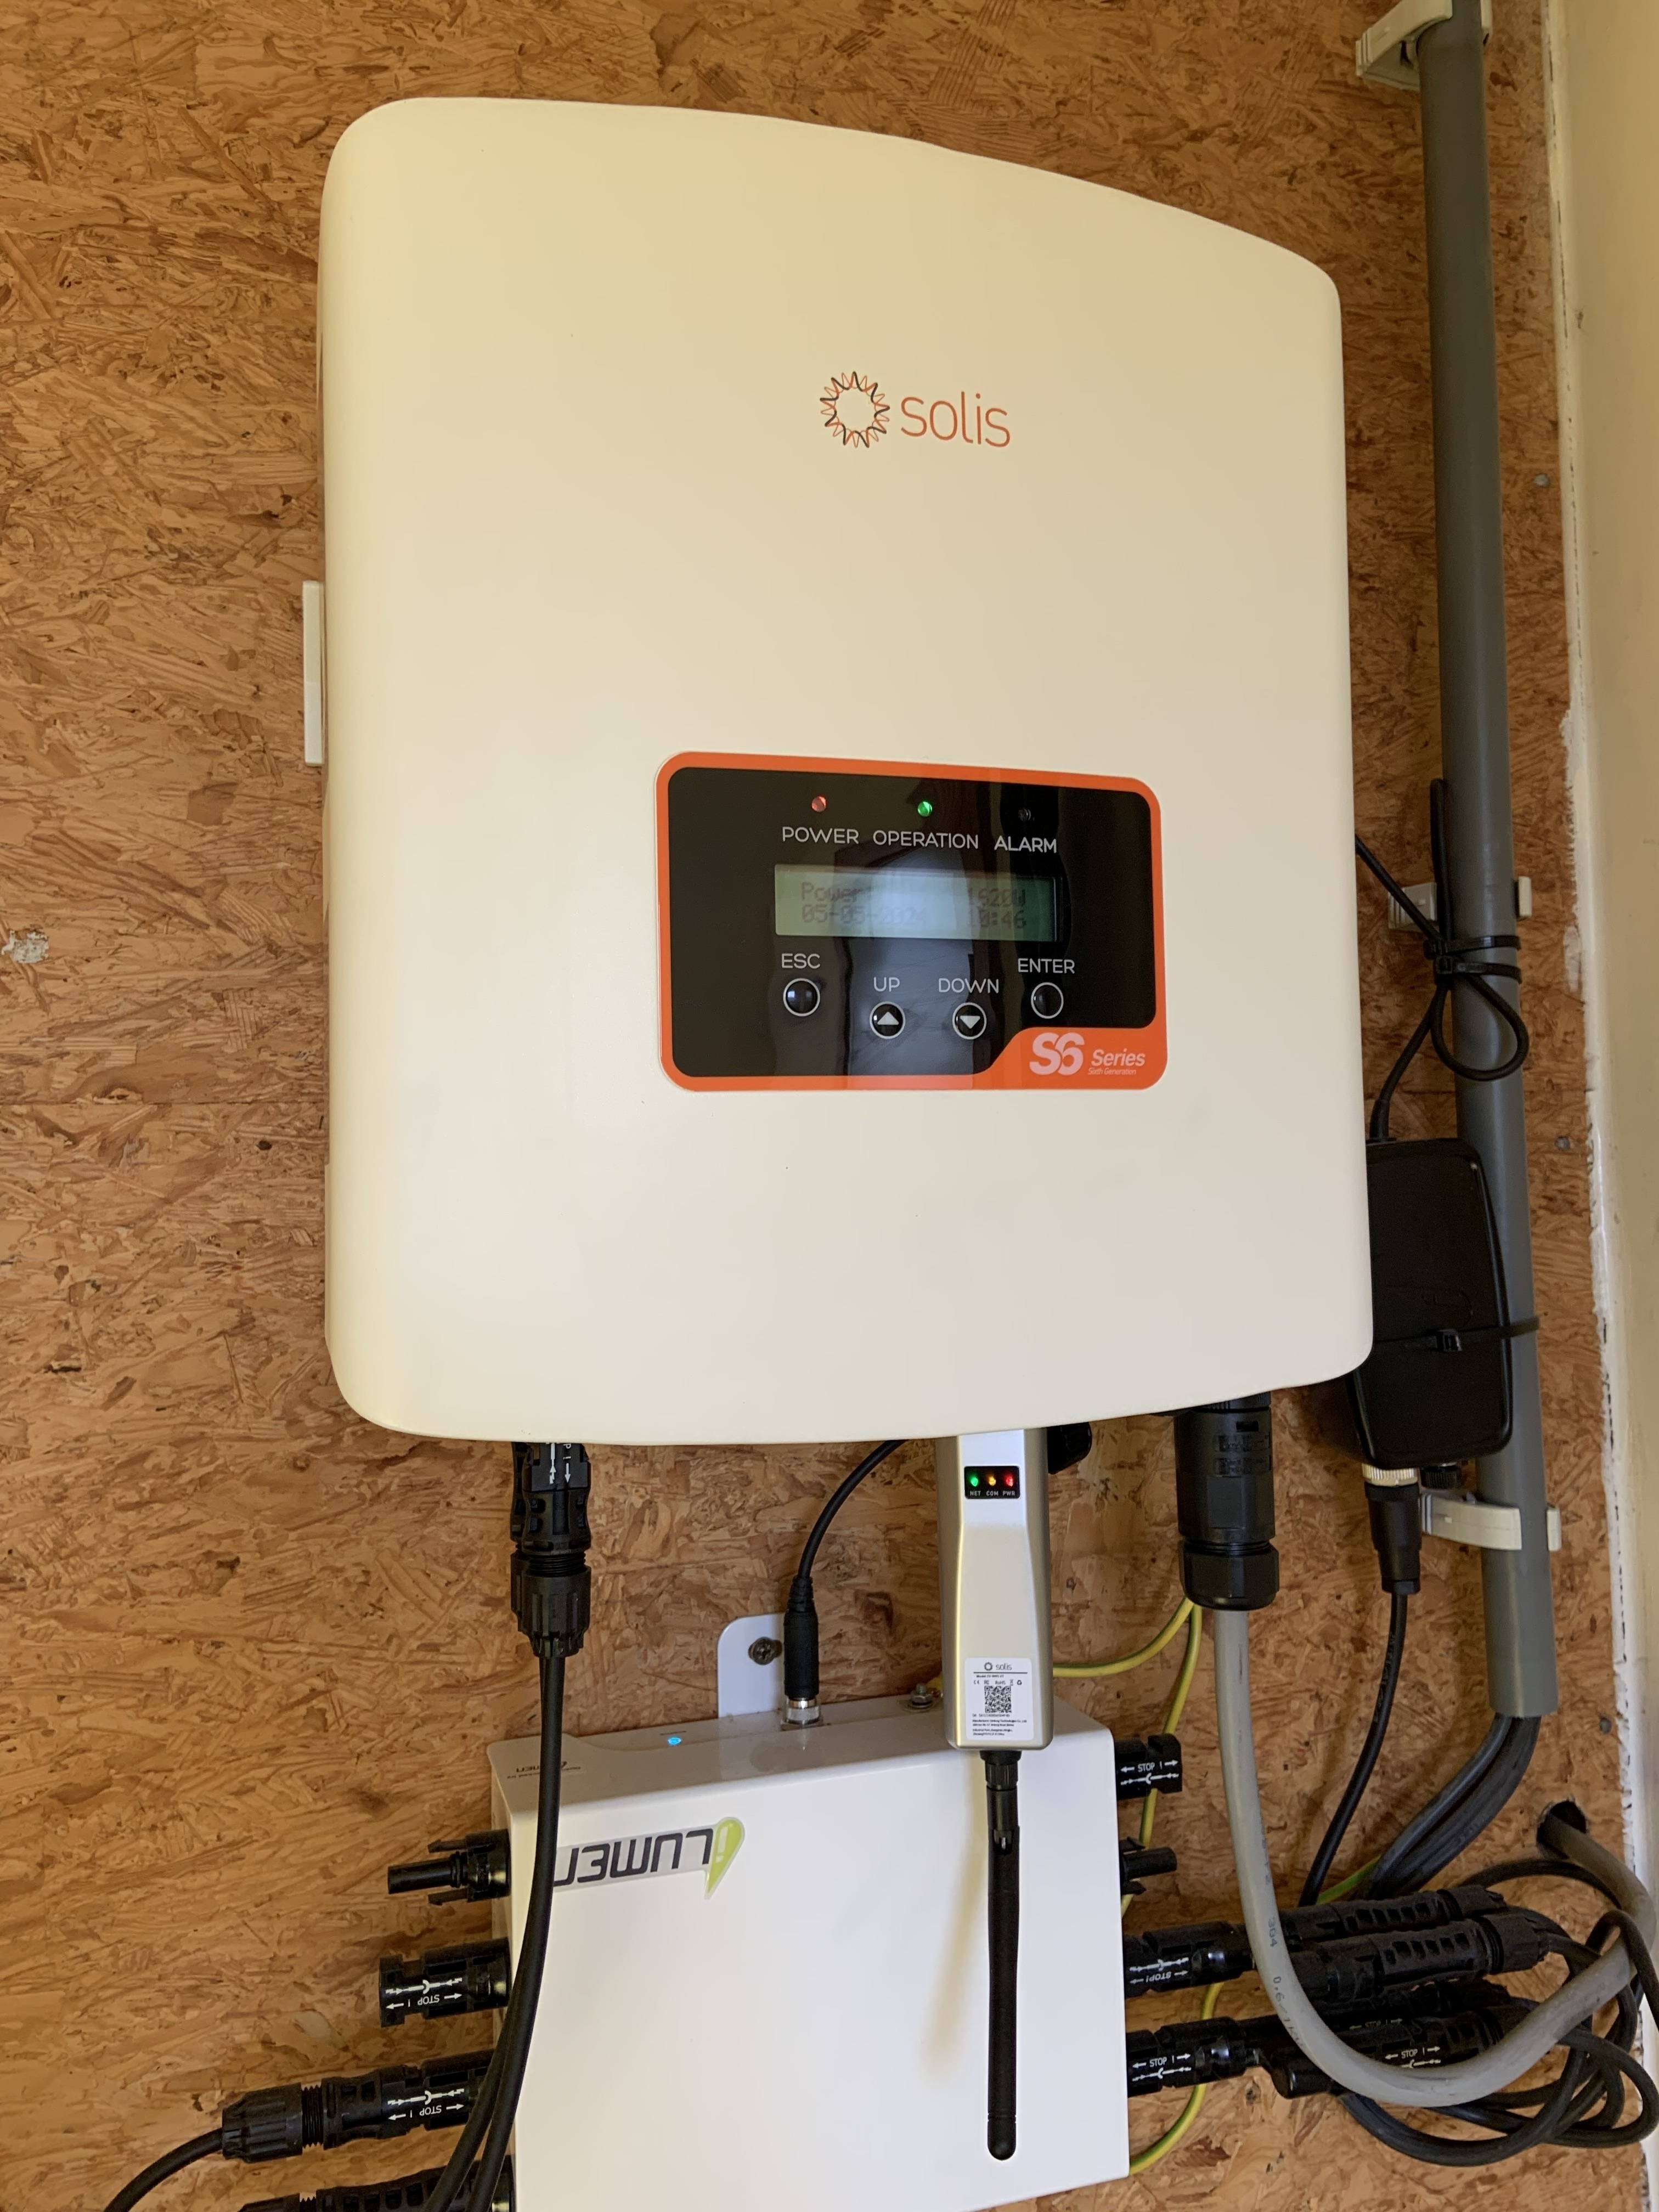
\includegraphics[width=7cm]{Omvormer} \hspace{0.5cm}
    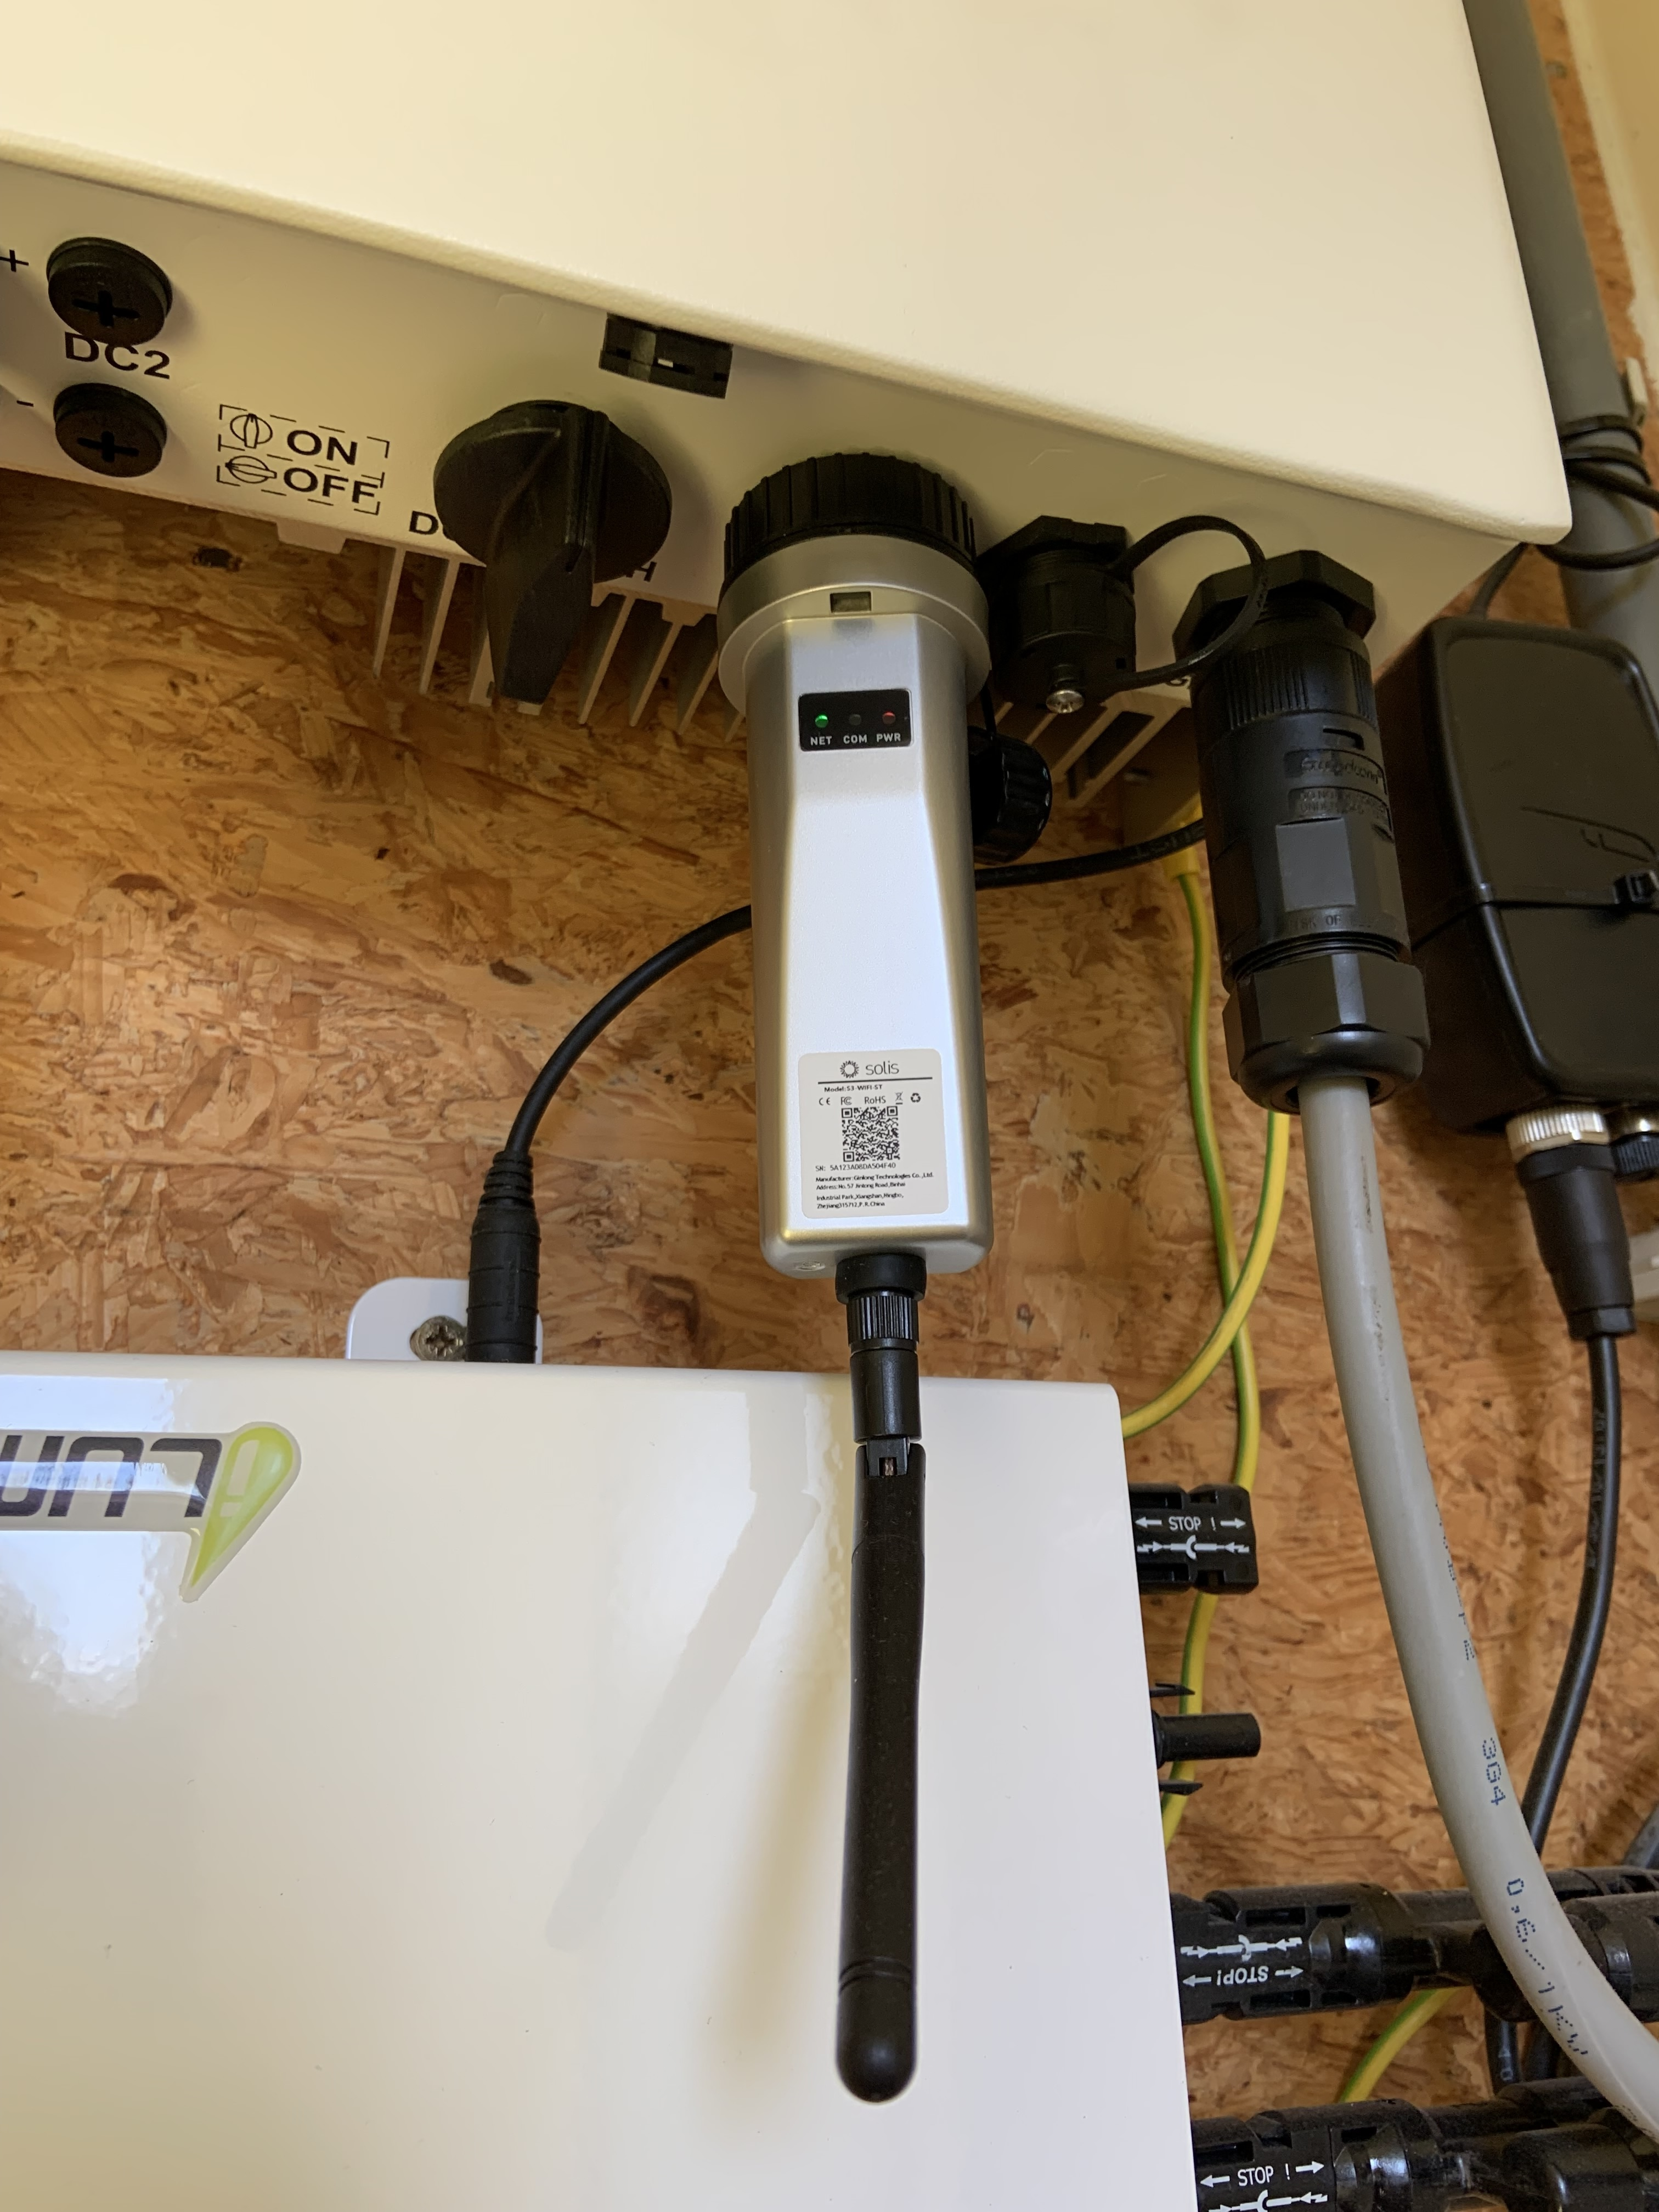
\includegraphics[width=7cm]{Wifi_Stick}
    \caption{Omvormer van de zonnepanelen met een wifi-stick.}
\end{figure}

Ook de data van de omvormer worden via het Python script weggeschreven naar een aparte InfluxDB databank en opgezet als een achtergrond service via de systeem manager voor Linux 'systemctl/systemd'. Zo blijft ook dit script automatisch uitgevoerd worden.

\subsection{\IfLanguageName{dutch}{Stroomproductie van zonnepanelen voorspellen met XGBoost}{Predicting power production PV system with XGBoost}}%
\label{sec:Stroomproductie van zonnepanelen voorspellen met XGBoost}

Het oorspronkelijke idee was om de stroomproductie van de zonnepanelen te gaan voorspellen op basis van de historische data van die stroomproductie. Voor dit onderzoek was er echter geen of slechts beperkte historische data voorhanden, omdat de metingen van de omvormer van de zonnepanelen pas gestart zijn bij het begin van het onderzoek. Na uitgebreid literatuuronderzoek werd beslist om de stroomproductie van de zonnepanelen te gaan voorspellen op basis van de hoeveelheid zonnestraling  \autocite{Sehrawat2023}, \autocite{Ledmaoui2023}, \autocite{Wang2022} en \autocite{Sansine2023}. Via de CAMS Radiation Service (CRS) van de Copernicus Atmosphere Monitoring Service (\href{https://atmosphere.copernicus.eu}{CAMS}) kan voldoende betrouwbare historische data met betrekking tot zonnestraling verkregen worden.

\subsubsection{Historische zonnestralingsdata verzamelen}

De zonnestralingsdata die via de CAMS Radiation Service (CRS) kan bekomen worden omvat tijdreeksen van globale, directe en diffuse instraling voor een tijdspanne van 1 februari 2004 tot en met 2 dagen geleden. De granulariteit van de data varieert van 1 maand tot 1 minuut en kan via een API-request opgevraagd worden. \\

Er bestaat een open source Python library 'pvlib' \autocite{Jensen2023} die ontwikkeld werd om de opbrengst van zonnepanelen te simuleren. Deze library bevat ook tools om zonnestralingsdata op te vragen, waaronder de data van de CAMS Radiation Service (CRS). Omdat de reeds ontwikkelde scripts voor het uitlezen van de digitale elektriciteitsmeter en de omvormer van de zonnepanelen in Python geschreven zijn, worden ook de andere scripts in Python geschreven en kan de pvlib library dus gebruikt worden. Om de zonnestralingsgegevens op te vragen moeten een aantal parameters worden meegegeven, waaronder de locatie (lengte- en breedtegraad), de start- en einddatum en de tijdsgranulariteit. Omdat van de gebruiker van de app niet kan verwacht worden dat hij of zij de geografische coördinaten van zijn of haar woning kent, wordt de Python library Geopy gebruikt om het ingevoerde adres van een gebruiker om te zetten in de correcte lengte- en breedtegraad  coördinaten en deze vervolgens mee te geven in de API-call naar de CRS. \\

Voor dit onderzoek wordt de zonnestralingsdata voor een periode van iets meer dan 5 jaar opgevraagd, van 1 januari 2019 tot op heden om precies te zijn. Dat heden is evenwel de datum van 2 dagen eerder, aangezien het 2 dagen duurt vooraleer de CRS de waargenomen zonnestralingsdata verwerkt en opgeslagen heeft. Dit geeft voldoende data om via een machine learning algoritme de toekomstige hoeveelheid zonnestraling te gaan voorspellen. Voor de granulariteit werd geopteerd voor metingen om de 15 minuten. Zo zijn de metingen van de bekomen dataset voldoende gedetailleerd om accurate voorspellingen te kunnen maken, zonder dat de performantie in het gedrang komt. Bij metingen van 1 minuut blijkt de dataset te omvangrijk om er op een efficiënte en dus snelle manier berekeningen op uit te voeren.

\begin{figure}[h!]
    \centering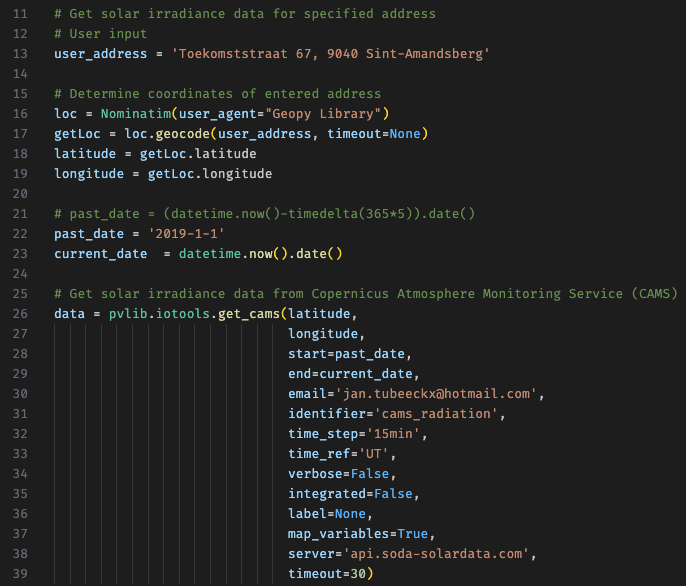
\includegraphics[scale=0.6]{Solar_Irradiance}
    \caption{\label{fig:Solar_Irradiance}Script voor het opvragen van de zonnestralingsdata.}
\end{figure} 

\subsubsection{Weerdata}

Niet alleen de hoeveelheid zonnestraling is bepalend voor de stroomproductie van zonnepanelen, ook de weersomstandigheden oefenen een invloed uit. Vooral de omgevingstemperatuur, de relatieve luchtvochtigheid en de bewolkingsgraad zijn factoren die de stroomproductie van zonnepanelen kunnen vergroten of verkleinen \autocite{Sehrawat2023}. \\

Om de voorspelling van de toekomstige stroomproductie van de zonnepanelen accurater te maken, zal de zonnestralingsdata in de eerste plaats gecombineerd worden met historische weerdata voor dezelfde periode, van 1 januari 2019 tot op heden. Ook hiervoor werd gezocht naar een open source API, waarmee de data via een Python script kan worden opgevraagd. Finaal is voor \href{https://dev.meteostat.net/}{Meteostat} gekozen. Deze API biedt een Pyhon library waarmee met slechts een enkele HTTP-request historische weerdata voor een bepaalde locatie kan worden opgevraagd. Meteostat verzamelt historische weer- en klimaatdata van weerstations en verschillende nationale meteorologische instituten van over de hele wereld. Omdat ook voor deze API-call de lengte- en breedtegraad van de gevraagde locatie moet worden ingegeven, wordt opnieuw gebruik gemaakt van de Python library Geopy waarmee een adres kan worden omgezet in de correcte lengte- en breedtegraad coördinaten. \\

\begin{figure}[h!]
    \centering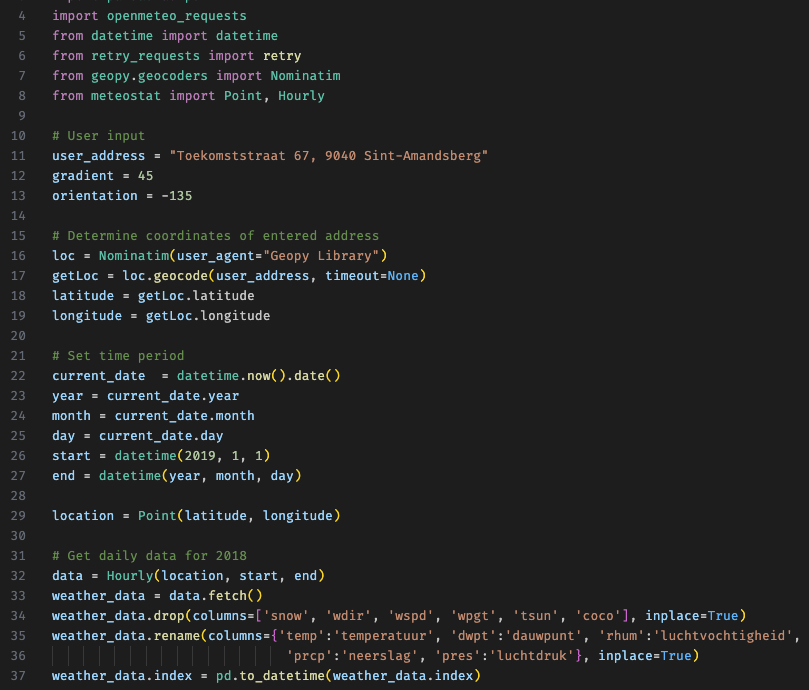
\includegraphics[scale=0.5]{Weerdata}
    \caption{\label{fig:Weerdata}Script voor het opvragen van de weerdata.}
\end{figure} 

Om de voorspelling van de stroomproductie van de zonnepanelen nog beter te maken, zal de bekomen voorspelling gecombineerd worden met de weersvoorspellingen voor de voorspelde periode. Aangezien Meteostat enkel historische data aanbiedt, moest een andere open source weer API gevonden worden. \href{https://open-meteo.com/}{Open-Meteo API} werkt ook samen met verschillende nationale meteorologische diensten waardoor het betrouwbare weersvoorspellingen aanbiedt. De aangeboden API-request is makkelijk in te stellen, zodat enkel de benodigde weerdata kan worden opgevraagd. Zo kan de data snel opgevraagd worden. Voor dit onderzoek worden enkel de voorspellingen van de omgevingstemperatuur, de relatieve luchtvochtigheid en de bewolkingsgraad opgehaald.

\subsubsection{Voorspelling met XGBoost}

Door het toenemend belang van hernieuwbare energie is er al heel wat onderzoek verricht naar het voorspellen van de elektriciteitsproductie van PV-systemen door toepassing van machine learning. Uit de meest recente onderzoeken blijkt dat Extreem Gradient Boosting (XGBoost) andere machine learning algoritmes overtreft bij het voorspellen van historische zonnestraling \autocite{Khasawneh2024}, \autocite{Tercha2024},  \autocite{Ledmaoui2023}, \autocite{Wang2022} en \autocite{BarreraAnimas2022}. Om die reden wordt voor dit onderzoek gebruik gemaakt van XGBoost om de toekomstige zonnestraling en vervolgens de stroomproductie van zonnepanelen te voorspellen. 

\subparagraph{Data cleaning en correlaties}
De dataset die als invoer voor het XGBoost algoritme gebruikt werd, is dus een combinatie van historische zonnestralingsdata en weerdata. Deze datset werd eerst gezuiverd van anomalieën door alle negatieve en ontbrekende waarden te verwijderen, anders zouden deze fouten de voorspelde waarden kunnen vertekenen. Na het opschonen van de data werden bestaande correlaties onderzocht. Hiervoor werd de Python library 'Seaborn' gebruikt, waarmee een heatmap van de correlaties tussen de verschillende kenmerken van de dataset kon worden opgemaakt. Daaruit blijkt inderdaad dat vooral de omgevingstemperatuur (positief) en luchtvochtigheid (negatief) het sterkst correleren met de globale horizontale instraling van de zon (GHI). 

\begin{figure}[h!]
    \centering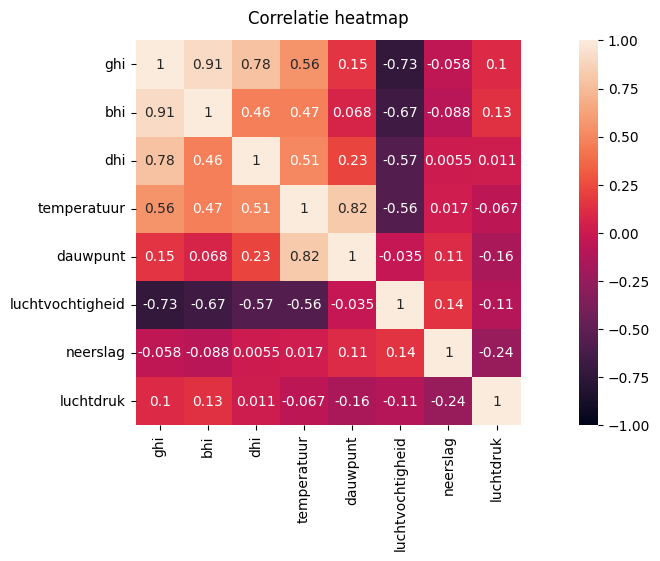
\includegraphics[scale=0.7]{correlatie}
    \caption{\label{fig:correlatie}Heatmap van correlaties tussen de verschillende kenmerken van de dataset.}
\end{figure} 

\newpage
\subparagraph{Toevoeging van features}
De historische zonnestralingsdata die gebruikt wordt, kan beschouwd worden als tijdreeksen (time series) vermits de data geordend is volgens een tijdsindex. Om de analyse van deze tijdreeksen te verbeteren en patronen in de zonnestralingsdata vast te stellen, worden extra 'Features' of tijdgerelateerde kenmerken  toegevoegd aan de gebruikte dataset. Deze kenmerken worden afgeleid van de index van de dataset die uit het tijdstip van de gemeten waarde bestaat (zie figuur 4.6). Deze verrijking zorgt voor een beter begrip van de tijdsgebonden aspecten van de gegevens en het later toegepaste XGBoost model bij het herkennen van patronen en seizoensgebondenheid.  

\begin{figure}[h!]
    \centering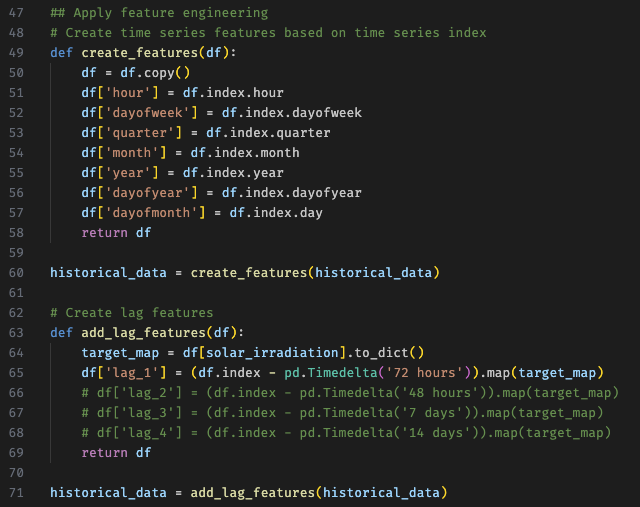
\includegraphics[scale=0.6]{Features_Lags}
    \caption{\label{fig:Features_Lags}Screenshot van de Python code voor het aanmaken van features en lags.}
\end{figure} 

\subparagraph{Toevoeging van lag features}
Om het XGBoost algoritme nog beter in staat te stellen om tijdsgebonden afhankelijkheden en verbanden te herkennen, worden zogenaamde 'lag features' of vertragingskenmerken aan de dataset toegevoegd. Hiermee wordt het algoritme opgedragen om de zonnestralingswaarden van een bepaald aantal dagen in het verleden op te nemen als nieuwe features. De toevoeging van lag features zorgt opnieuw voor een verrijking van de dataset en voorziet het model van historische informatie om zonnestralingspatronen beter te begrijpen en te voorspellen, wat uiteindelijk bijdraagt aan de nauwkeurigheid en effectiviteit van het XGBoost model \autocite{Nabatchian2024}.

\subparagraph{XGBoost model trainen en testen}
Omdat het XGBoost model heel wat parameters bevat die kunnen aangepast worden, werden verschillende versies ontwikkeld en getest. Om elke versie te kunnen beoordelen werd de gebruikte dataset opgesplitst in een trainingset en een testset. Daarbij werd het algoritme getraind op de trainigset en beoordeeld op testset. Omdat de data uit tijdreeksen bestaat, werd voor het opsplitsen van de dataset geopteerd voor de 'TimeSeriesSplit' functie van de Scikit-learn library. Deze functie is speciaal ontworpen voor de opsplitsing van tijdreeksgegevens en zorgt ervoor dat de chronologische volgorde van de gegevens behouden blijft tijdens het opsplitsingsproces. Dit zorgt voor een grotere nauwkeurigheid van de beoordeling van de voorspellingscapaciteit van het model.

\begin{figure}[h!]
    \centering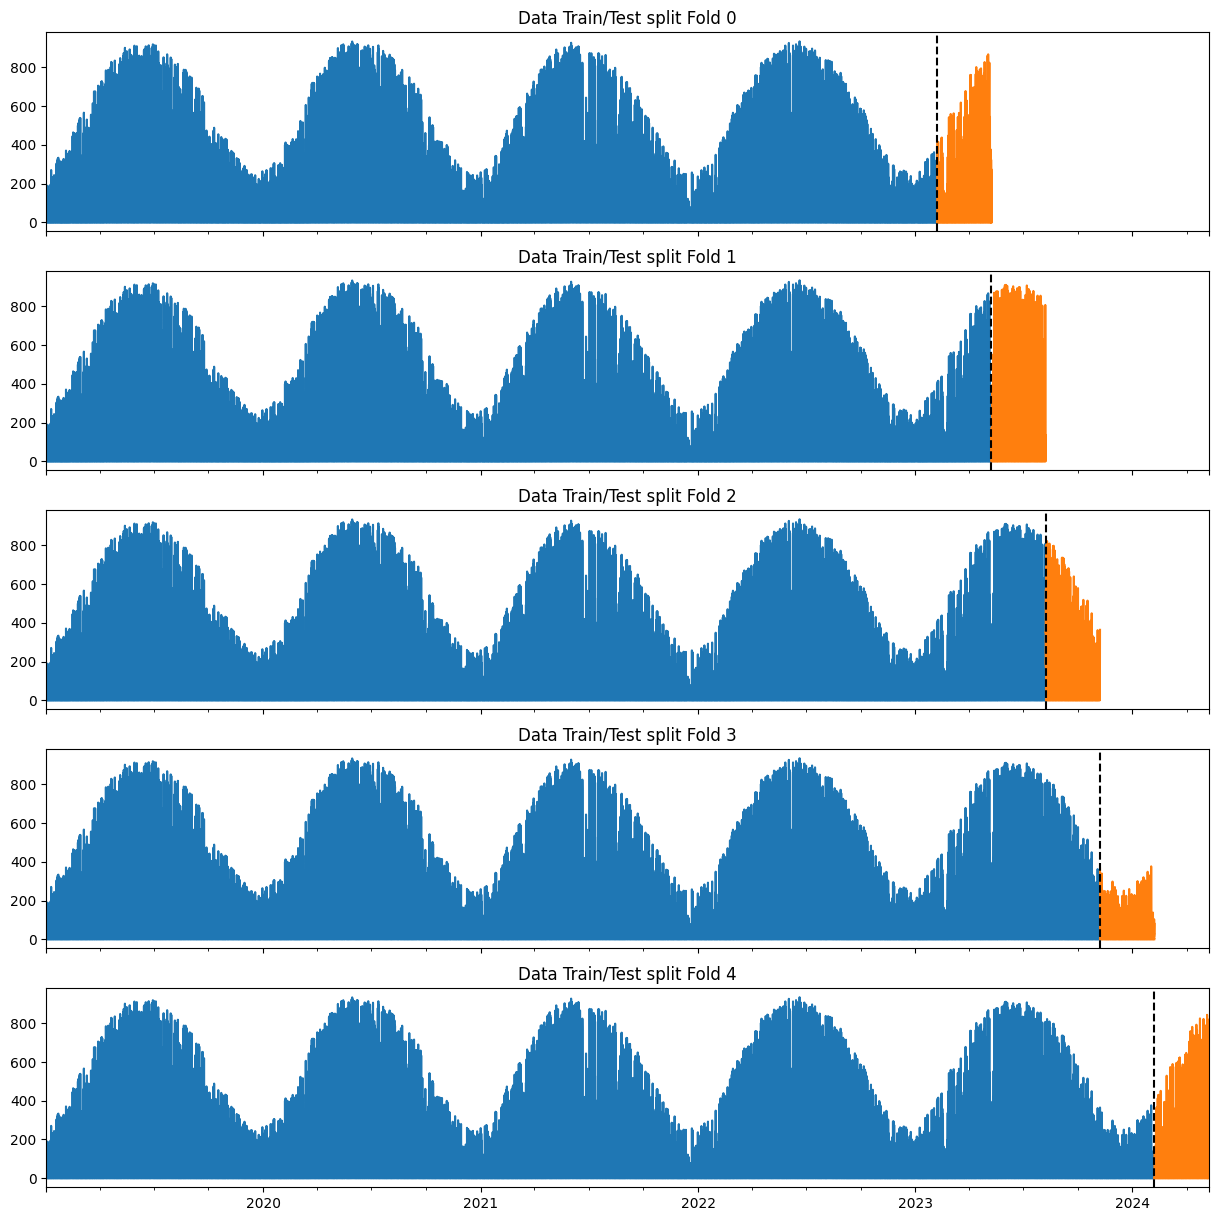
\includegraphics[scale=0.45]{TimeSeriesSplit}
    \caption{\label{fig:TimeSeriesSplit}Grafische voorstelling van de TimeSerieSplit functie.}
\end{figure} 

Om de geteste modellen te beoordelen werd telkens de mean absolute error (MAE), mean squared error (MSE) en root mean squared error (RMSE) over de verschillende opsplitsingen heen berekend. Het uiteindelijk gekozen model behaalde volgende scores: MAE score van 0.5519, MSE score van 1.5816 en RMSE score van 1.2576.

\subparagraph{Voorspelling van de zonnestraling}

Om de toekomstige zonnestaling te voorspellen werd het geselecteerde algoritme getraind op de volledige dataset met alle historische data, zonder een opsplitsing te maken tussen een training- en testset. De bekomen voorspelling van de zonnestraling werd vervolgens gecombineerd met de voorspelling van de omgevingstemperatuur en de relatieve luchtvochtigheid die via de Open-Meteo API voor dezelfde periode werd opgehaald. 

\begin{figure}[h!]
    \centering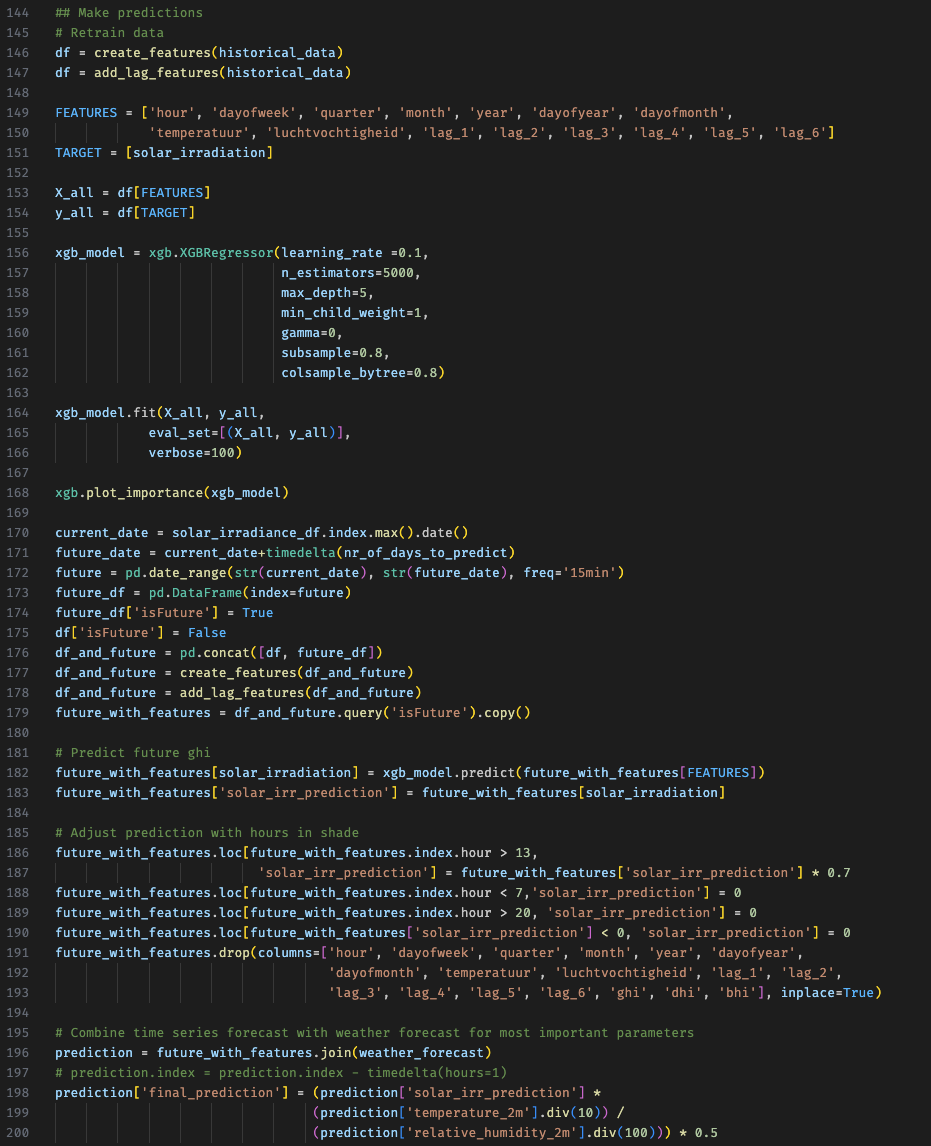
\includegraphics[scale=0.42]{Prediction}
    \caption{\label{fig:Prediction}Screenshot van de Python code voor de voorspelling van de zonnestraling van de volgende dag.}
\end{figure} 

\newpage
\subparagraph{Omzetting voorspelde zonnestraling naar opgewekte stroom}

Op basis van de gecombineerde voorspelling van de zonnestraling (GHI) kan vervolgens de toekomstige stroomproductie van de zonnepanelen berekend worden. Daarbij geldt dat het opgewekte vermogen van zonnepanelen lineair toeneemt naarmate de zonnestraling (GHI) toeneemt, en lineair afneemt naarmate de omgevingstemperatuur toeneemt. Het opgewekte vermogen van de zonnepanelen kan dan berekend worden door de formule

\begin{figure}[h!]
    \centering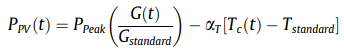
\includegraphics[scale=0.7]{PVPower_Formula}
\end{figure} 

waarbij 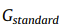
\includegraphics[height=1.7em]{Gstandard} en 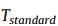
\includegraphics[height=1.7em]{Tstandard} verwijzen naar de standaard testcondities die fabrikanten van zonnepanelen hanteren \autocite{Kazem2017}. Deze standaard test condities zijn 1000 W/m² zonnestraling en een omgevingstemperatuur van 25\textdegree C. \\ 

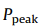
\includegraphics[height=1.7em]{PPeak} verwijst naar het piekvermogen van de zonnepanelen. Dit piekvermogen(Wp) wordt onder bovenstaande omstandigheden door de fabrikant bepaald. \\

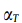
\includegraphics[height=1.5em]{Temp_Coeff} verwijst naar de temperatuur-coëfficiënt. Deze waarde geeft aan wat de invloed is van de temperatuur van de zonnepanelen op het rendement van de zonnepanelen. De meeste zonnepanelen hebben een temperatuurcoëfficiënt van ongeveer -0,35 \% per graad Celsius. Dat betekent dat het vermogen ongeveer met 1\% afneemt bij een stijging van 3 graden Celsius. \\

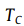
\includegraphics[height=1.5em]{Cell_Temp} tenslotte verwijst naar de zonneceltemperatuur en word berekend via volgende fomule:

\begin{figure}[h!]
    \centering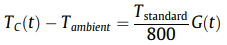
\includegraphics[scale=0.7]{CellTemp_Formula}
\end{figure} 

De PV-installatie die voor dit onderzoek gebruikt werd, bestaat uit 10 zonnepanelen die elk een piekvermogen van 215 Watt hebben. Dit geeft een totaal piekvermogen van 2.150 Watt. Zonnepanelen behalen echter nooit hun volledige piekvermogen omdat de weers- en omgevingsfactoren anders zijn dan de bovenvermelde standaard testcondities die door de fabrikanten gebruikt worden. In België moet rekening gehouden worden met een omgevingsfactor van 0,85. Dit betekent dat het werkelijke piekvermogen van de zonnepanelen slechts 1.827,50 Watt is (2.150 Watt x 0,85). De zonnepanelen die in dit onderzoek gebruikt werden, zijn echter al 25 jaar oud en uit de metingen gedurende anderhalve maand blijkt dat zij nog maar 76\% van hun piekvermogen halen, zijnde 1.634 Watt. \\

Omdat de historische zonnestralingsdata van de CAMS Radiation Service (CRS) van de Copernicus Atmosphere Monitoring Service (\href{https://atmosphere.copernicus.eu}{CAMS}) met 2 dagen vertraging verkregen wordt, kon de accuraatheid van de gemaakte voorspelling makkelijk geverifieerd worden. Vermits de gegevens van de stroomproductie van de PV-installatie in real time werden uitgelezen, konden deze gegevens op het einde van de dag vergeleken worden met de voorspelling. Daaruit bleek telkens dat de gemaakte voorspelling de effectieve stroomproductie dicht benaderde, zoals uit onderstaande figuur blijkt.

\begin{figure}[h!]
    \centering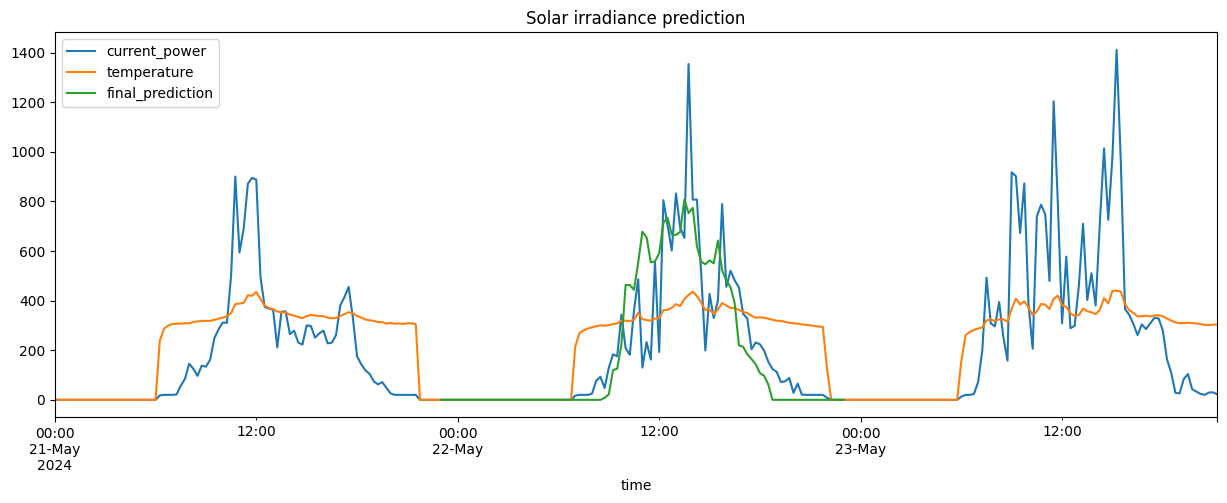
\includegraphics[scale=0.5]{power_prediction}
    \caption{\label{fig:power_prediction}Vergelijking van de effectieve stroomproductie (blauw) met de voorspelde stroomproductie (groen).}
\end{figure} 

\subsection{\IfLanguageName{dutch}{Weergave uitgelezen data en voorspelling met een iOS app}{Display of data and prediction with an iOS app}}%
\label{sec:Weergave uitgelezen data en voorspelling met een iOS app}

Omdat een smartphone makkelijker en vaker consulteerbaar is, werd in dit onderzoek geopteerd voor de ontwikkeling van een mobiele app om de elektriciteitscon- sumptie- en productie weer te geven en op te volgen. De app is ontwikkeld voor iOS omdat dit het testen achteraf vergemakkelijkt. De iOS-app werd gebouwd in de geïntegreerde ontwikkelomgeving (IDE) XCode met SwiftUI en UIKit. Voor documentatie en tutorials werd gebruik gemaakt van het \href{https://developer.apple.com/}{Apple developer platform}. \\

Om de uitgelezen data van de digitale elektriciteitsmeter en de omvormer van de zonnepanelen beschikbaar te maken voor de app, werd eerst een webserver geïnstalleerd op de Raspberry Pi. Daarvoor werd Flask gebruikt. Dit is een open source Python web framework, waarmee op een eenvoudige manier webapplicaties gebouwd kunnen worden. Het is een micro-framework wat betekent dat het weinig tot niet afhankelijk is van externe libraries en zeer licht is. Omdat de backend voor de ontwikkelde app eerder beperkt is en de webserver op een minicomputer moet draaien, is Flask de meest voor de hand liggende keuze \autocite{Shokrzad2023}. Met de toevoeging van één enkel bijkomend Python bestand konden alle nodige REST-calls opgezet worden. 

\subsubsection{Elektriciteitsconsumptie en -productie}
De ontwikkelde app geeft de gebruiker vooreerst een overzicht van zijn of haar elektriciteitsverbruik- en productie. 

\begin{figure}[h!]
    \centering
    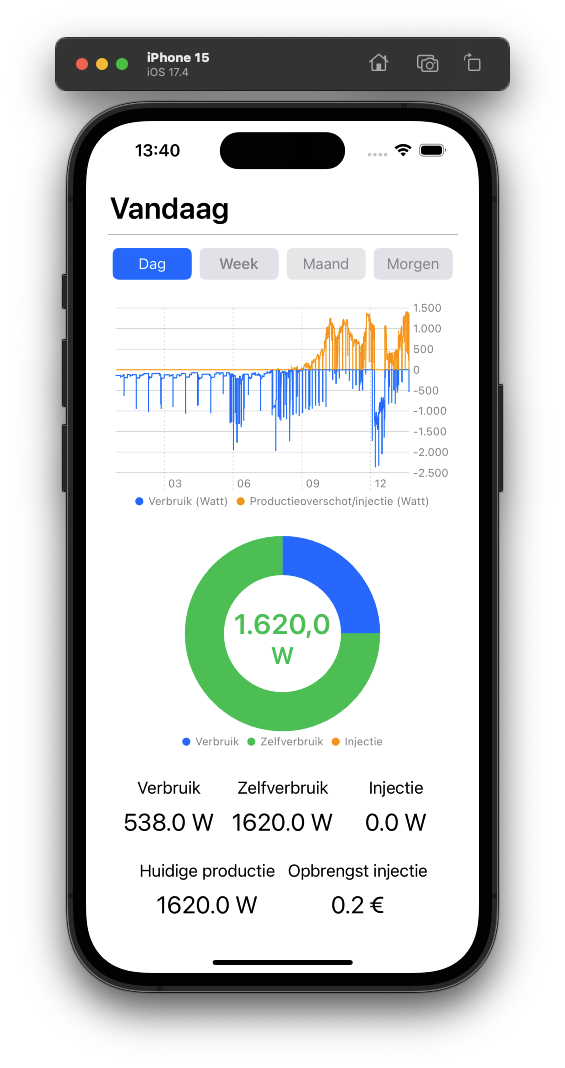
\includegraphics[width=5cm]{Iphone_dag_cons} \hspace{0.1cm}
    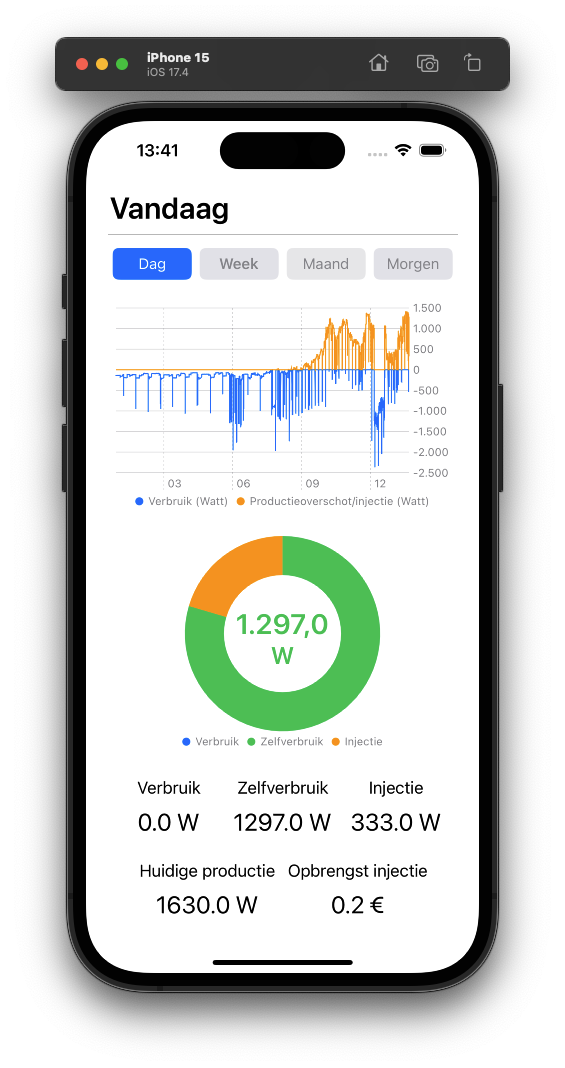
\includegraphics[width=5cm]{Iphone_dag_self} \hspace{0.1cm}
    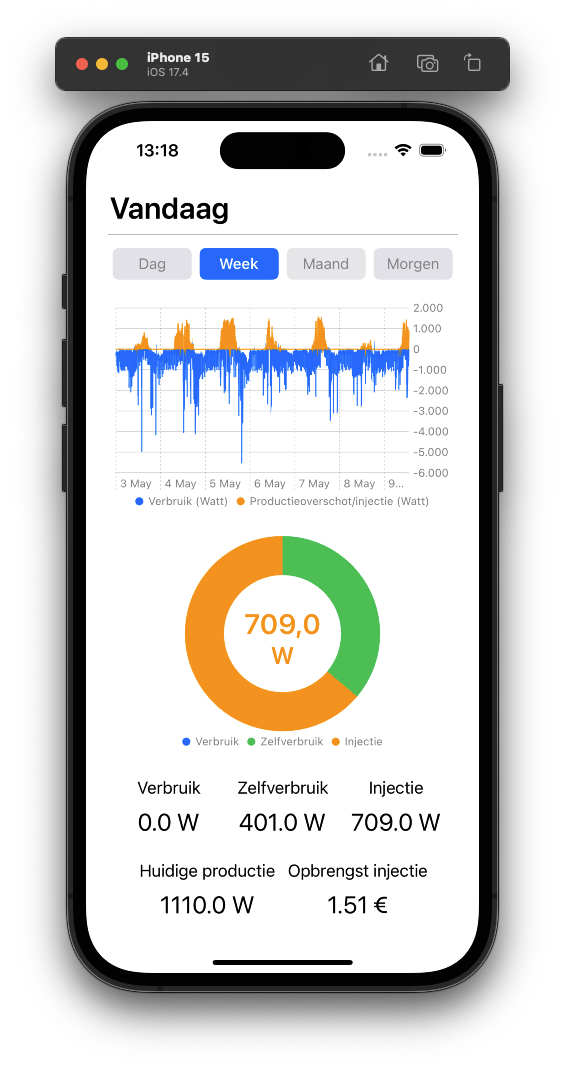
\includegraphics[width=5cm]{Iphone_week}
    \caption{Overzicht elektricteitsverbruik en -productie per dag en per week.}
\end{figure}

Op een eerste grafiek worden per periode (dag, week, maand) het verbruik en productieoverschot getoond. Dit productieoverschot is de zelf geproduceerde stroom die niet verbruikt wordt en dus in het distributienetwerk geïnjecteerd wordt. Voor deze injectie ontvangt de gebruiker een beperkte vergoeding van zijn of haar stroomleverancier. Het doel van het onderzoek van deze bachelorproef is niet enkel om het elektriciteitsverbruik beter te gaan spreiden, maar ook om ervoor te zorgen dat de zelf geproduceerde stroom van de zonnepanelen effectief zelf verbruikt wordt. Het bedrag van de vergoeding voor de geïnjecteerde stroom is immers dermate laag dat het financieel voordeliger is om de zelfgeproduceerde elektriciteit zelf te gebruiken, dan deze stroom te verkopen. Om die reden wordt het bedrag van de opbrengst van de geïnjecteerde stroom gedurende de geselecteerde periode aan de gebruiker getoond. Zo heeft deze een besef van het voordeel dat het zelfverbruik hem of haar oplevert. \\

Op een tweede grafiek worden de huidige consumptie- en productiegegevens getoond. Zo ziet de gebruiker duidelijk hoeveel elektriciteit hij of zij van het net afneemt en dus betaalt, hoeveel van de zelf opgewekte stroom hij of zij effectief zelf gebruikt en hoeveel van de zelfgeproduceerde stroom geïnjecteerd en dus verkocht wordt. Daarbij wordt in het midden van de grafiek de grootste van deze drie waarden getoond, zodat de gebruiker meteen ziet wat er overheerst: zijn of haar verbruik, zelfconsumptie of injectie. \\

Tot slot worden onder de beide grafieken de consumptie- en productiedetails als waarden getoond. Zo ziet de gebruiker ook de totale hoeveelheid elektriciteit die door de zonnepanelen wordt opgewekt.

\subsubsection{Voorspelling stroomproductie}

Via de app kan ook de voorspelde stroomproductie van de volgende dag geraadpleegd worden. Deze voorspelling is het resultaat van het Python script waarmee het XGBoost algoritme en de voorspelling van de stroomproductie geïmplementeerd werd. Dit script wordt automatisch om het uur uitgevoerd, zodat steeds een recente voorspelling kan getoond worden. De gemaakte voorspelling wijzigt immers doorheen de dag. Het is op basis van deze voorspelling dat de app automatisch sanitaire of andere apparaten zal gaan inschakelen wanneer er voldoende stroomproductie voorspeld wordt. 

\begin{figure}[h!]
    \centering
    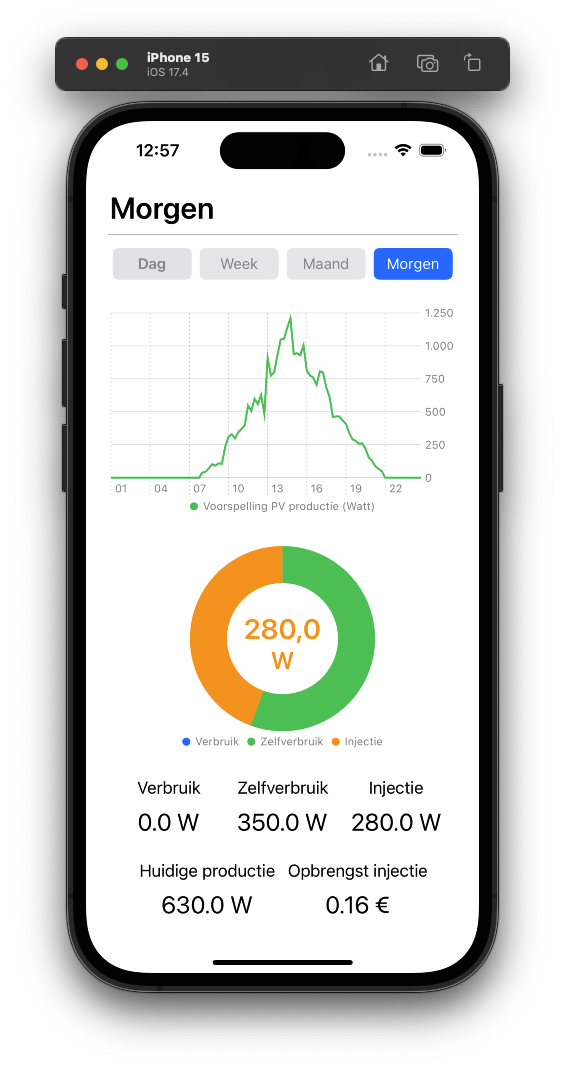
\includegraphics[width=5cm]{Iphone_prediction} \hspace{0.5cm}
    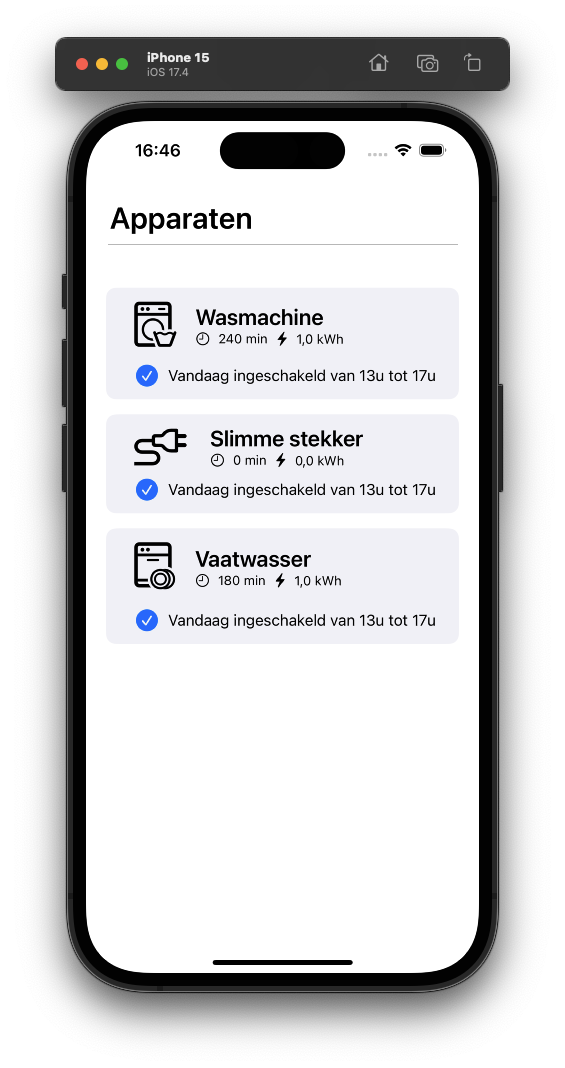
\includegraphics[width=5cm]{Device_List}
    \caption{Voorspelling van de stroomproductie en overzicht van de ingeschakelde apparaten.}
\end{figure}

\newpage
\subsection{\IfLanguageName{dutch}{Aansturing slimme apparaten op basis van de voorspelde stroomproductie}{Predicting power production PV system with XGBoost}}%
\label{sec:Aansturing slimme stekkers aansturen op basis van de voorspelde stroomproductie}

De gebruiker zal via de app toestellen kunnen toevoegen die automatisch ingeschakeld mogen en kunnen worden wanneer er voldoende stroomproductie voorspeld wordt. De app zal de gebruiker adviseren over welke apparaten het best kunnen worden toegevoegd omdat ze het meeste verbruiken. Denk daarbij in de eerste plaats aan een warmtepomp of laadpaal indien deze aanwezig zijn, maar ook aan de wasmachine en de vaatwasser. De app zal zelf het verbruik en de inschakelduur van het apparaat gaan bepalen. Indien bijvoorbeeld een wasmachine wordt toegevoegd, dan zal de app het verbruik instellen op 1 kWh en ervan uitgaan dat een wasprogramma gemiddeld 3 uur duurt. De gebruiker zal evenwel de mogelijkheid hebben om dit verbruik en de inschakeltijd zelf te gaan instellen, net zoals hij de mogelijkheid heeft om de inschakeling van een apparaat handmatig te verhinderen.\\

Wanneer uit de voorspelling van de stroomproductie blijkt dat er voldoende elektriciteit zal worden opgewekt de volgende dag, zal de app de door de gebruiker toegevoegde toestellen gaan inplannen voor de volgende dag. Dit was althans de theorie, want bij de selectie van de toestellen voor dit onderzoek bleek dat de toestellen van het huis dat als testomgeving diende nog niet 'slim' waren. Een probleem dat zich helaas zal voordoen bij heel wat gezinnen. Om dit op te vangen werd gebruik gemaakt van slimme stekkers. Dit zijn stekkers die via wifi kunnen in- en uitgeschakeld worden. Zij worden tussen het klassieke stopcontact en de stekker van het toestel geplaatst, waardoor een toestel op een eenvoudige manier slim kan gemaakt worden \autocite{Jong2020}. Maar ook daarbij stelde zich een probleem. Een slimme stekker kan enkel stroom doorlaten of tegenhouden. Dit vereist dat een toestel reeds kan ingeschakeld worden indien het geen stroom krijgt en dat het dus zonder tussenkomst van een gebruiker kan opstaren van zodra de slimme stekker stroom doorlaat. De sanitaire toestellen van de testopstelling voor dit onderzoek, konden pas worden aangezet nadat ze stroom kregen én op een elektronische startknop geduwd werd. \\

Om de werking van de app in combinatie met slimme stekkers toch te testen, werd een slimme stekker verbonden met de batterijlader van een elektrische fiets. De aansturing van de slimme stekker gebeurt via een Python script dat als een service op de Raspberry Pi minicomputer uitgevoerd wordt. In dit script wordt de slimme stekker bestuurd met behulp van de Python library PyP100 die speciaal ontwikkeld werd voor het gebruikte merk van stekker. Via deze library kan verbinding gemaakt worden met de slimme stekker door het IP-adres en de inloggegevens mee te geven. \\

\begin{figure}[h!]
    \centering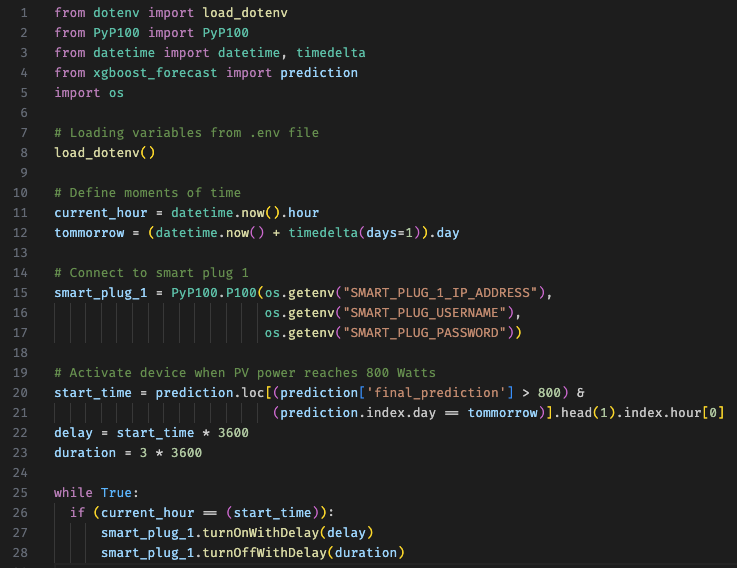
\includegraphics[scale=0.53]{SmartPlug_Script}
    \caption{\label{fig:SmartPlug_Script}Screenshot van de Python code om de slimme stekker aan te sturen op basis van de voorspelde stroomproductie.}
\end{figure} 

Het script is zo geprogrammeerd dat het elke dag om 23u wordt uitgevoerd. Het vraagt daarbij eerst de voorspelling van de stroomproductie van de volgende dag op. Vervolgens zal de slimme stekker geprogrammeerd worden om de volgende dag in te schakelen van zodra de voorspelde waarde van de opgewekte stroom 800 Watt of meer bedraagt. Op dat ogenblik zal eerst nog geverifieerd worden of de stroomproductie van de zonnepanelen effectief 800 Watt bedraagt. Is dit niet het geval, dan zal de slimme stekker niet ingeschakeld worden. Op de dag zelf kan de gebruiker in de app een overzicht kunnen raadplegen van de ingeschakelde apparaten met hun tijdschema.
%%=============================================================================
%% Conclusie
%%=============================================================================

\chapter{\IfLanguageName{dutch}{Conclusie}{Conclusion}}%
\label{ch:conclusie}

% TODO: Trek een duidelijke conclusie, in de vorm van een antwoord op de
% onderzoeksvra(a)g(en). Wat was jouw bijdrage aan het onderzoeksdomein en
% hoe biedt dit meerwaarde aan het vakgebied/doelgroep? 
% Reflecteer kritisch over het resultaat. In Engelse teksten wordt deze sectie
% ``Discussion'' genoemd. Had je deze uitkomst verwacht? Zijn er zaken die nog
% niet duidelijk zijn?
% Heeft het onderzoek geleid tot nieuwe vragen die uitnodigen tot verder 
%onderzoek?
Met deze bachelorproef werd getracht een antwoord te formuleren op de vraag of artificiële intelligentie kan worden aangewend om het elektriciteitsverbruik van gezinnen automatisch bij te sturen en zo de elektriciteitskosten te drukken. De behoefte aan dit onderzoek kwam er na de vaststelling dat heel wat gezinnen hun elektriciteitsconsumptie niet aanpassen wanneer ze over een app beschikken die hun energieverbruik en -productie enkel inzichtelijk maakt. Blijkbaar zorgt dit niet voor een gedragswijziging en was het dus nuttig om na te gaan hoe een app dan zelf het elektriciteitsverbruik kan bijsturen. Met andere woorden, kan een app door middel van artificiële intelligentie zo 'slim' gemaakt worden dat deze zelf apparaten in een gezinswoning kan in- of uitschakelen om zo het elektricteitsverbruik af te stemmen op de elektriciteitsproductie van de zonnepanelen? Het idee was om de stroomproductie van een PV-installatie te gaan voorspellen met behulp van machine learning om dan vervolgens slimme toestellen of slimme stekkers te gaan aansturen op basis van de gemaakt voorspelling. Dit zou worden uitgewerkt in zelf ontwikkelde app die als proof of concept zou dienen.\\

Om deze vraag te kunnen beantwoorden was vooreerst de juiste testomgeving noodzakelijk. Deze moest bestaan uit een woning met een digitale elektriciteitsmeter en een PV-installatie (zonnepanelen). Vervolgens moest werden nagegaan op welke manier een digitale elektriciteitsmeter en de omvormer van de PV-installatie op continue wijze konden worden uitgelezen. De oplossing hiervoor werd gevonden in de Raspberry Pi minicomputer. Dit toestel kon via wifi worden aangesloten op het thuisnetwerk van de woning die als testomgeving dienst deed. Vervolgens werden hierop Python scripts uitgevoerd die de gegevens van de elektriciteitsmeter en de omvormer van de zonnepanelen uitlazen en wegschreven naar een Influx databank. Gedurende de testperiode bleek deze oplossing zeer robuust en stabiel. Enige nadeel was dat wanneer het signaal van het wifinetwerk wegviel door een stroomonderbreking, het uitlezen gestopt werd. Dit werd uiteindelijk opgevangen door de Python scripts te voorzien van een automatisch heropstart commando. \\

Na het opzetten van de nodige hardware en het uitschrijven van de Python-scripts, werd onderzocht welke vorm van artificiële intelligentie kon worden aangewend om de voorspellingen van de stroomproductie te gaan maken. Na een uitgebreide literatuurstudie werd geopteerd voor de machine learning techniek van extreme gradient boosting (XGBoost). Deze methode is specifiek ontworpen om grootschalige datasets efficiënt te verwerken en leidt tot nauwkeurige voorspellingen. De toepassing van dit algoritme op de historische zonnestralingsdata van de afgelopen vijf jaar die via de CAMS Radiation Service (CRS) van de Copernicus Atmosphere Monitoring Service (\href{https://atmosphere.copernicus.eu}{CAMS}) verkregen werd, leidde inderdaad tot correcte voorspellingen. Om de gemaakte voorspelling nog nauwkeuriger te maken werd de historische zonnestralingsdata in de eerste plaats gecombineerd met historische weerdata. Uit onderzoek blijkt immers dat de temperatuur en luchtvochtigheid een invloed hebben op de elektricteitsproductie van zonnepanelen. Vervolgens werd de bekomen voorspelling gecombineerd met de weersvoorspelling voor de voorspelde periode. Zo kon dan een voldoende accurate voorspelling van de stroomproductie gemaakt worden. Om de uitgelezen elektricteitsgegevens en de voorspelling van de elektriciteitsproductie te visualiseren werd tenslotte een iOS app ontwikkeld. \\

De laatste stap van het onderzoek zou er dan in bestaan om de gemaakte voorspelling van de stroomproductie te gebruiken om (sanitaire) toestellen aan te sturen. Bij het formuleren van het onderzoeksvoorstel van deze bachelorproef werd ervan uitgegaan dat er een testomgeving beschikbaar zou zijn met zonnepanelen en een recente warmtepomp waarmee ook sanitair water wordt opgewarmd. Het is namelijk zo dat de huidige warmtepompen kunnen aangestuurd worden via een HEMS (home energy management system) en bijgevolg de ideale toestellen vormen om aan te sturen, zeker als ze ook gebruikt worden voor de opwarming van sanitair water. Zo kan de stroom van de zonnepanelen overdag immers gebruikt worden om het water in het boilervat van de warmtepomp op te warmen. De testomgeving die voor dit onderzoek gebruikt werd, beschikte echter niet over een warmtepomp. En al gauw bleek hier het grootste obstakel voor dit onderzoek. Andere toestellen in een gezinswoning die interessant zijn om via een HEMS aan te sturen, zijn een wasmachine en vaatwasser. Deze worden meestal op dagelijkse basis gebruikt en zijn tevens toestellen die redelijk wat energie verbruiken. Probleem is evenwel dat in de meeste gezinswoningen en ook in de woning van de testomgeving, deze toestellen niet 'slim' zijn en dus niet via wifi en een app kunnen worden aangestuurd. Als oplossing werd daarom teruggegrepen naar slimme stekkers. Daar stelde zich evenwel opnieuw een probleem. De huidige wasmachines en vaatwassers hebben meestal een elektronische startknop die enkel bediend kan worden als het toestel van elektriciteit voorzien wordt. Het toestel kan dus niet op zodanig wijze klaar gezet worden, dat het een wasprogramma start wanneer het stroom krijgt. De gebruiker zal nog steeds moeten tussenkomen om de startknop van het apparaat in te duwen. Hoewel dit voor het onderzoek van deze bachelorproef een probleem vormde, is de verwachting dat in de toekomst sanitaire toestellen standaard uitgerust zullen zijn met een wifiverbinding en dus via een app kunnen aangestuurd worden. Aandachtspunt daarbij zal zijn dat het op dit moment nog niet duidelijk is of daarbij een standaard communicatieprotocol zal gehanteerd worden, of dat elke fabrikant een eigen protocol blijft gebruiken. In het laatste geval zal de aansturing met een HEMPS-app een stuk moeilijker zijn omdat de app dan met al die verschillende communicatieprotocollen zal moeten kunnen omgaan. Dit maakt de ontwikkeling en het onderhoud ervan complexer. \\

Als alternatief werd in dit onderzoek gekozen voor de batterijlader van een elektrische fiets. Deze lader kon zonder problemen ingeschakeld worden met behulp van een slimmer stekker. De lader kon elke avond worden aangesloten en startte de volgende dag met opladen van zodra de zonnepalen een vermogen van 800 Watt produceerden. Deze grens van 800 Watt werd vastgelegd na een testperiode van 3 weken. Uit de vaststellingen bleek immers dat op deze manier gemiddeld het grootste aantal uren aan stroomproductie van een gemiddelde dag kon bekomen worden.  Er werd gedurende drie weken getest met deze opstelling en daaruit bleek dat de ontwikkelde app in staat was om de slimme stekker en dus de batterijlader op het correcte moment in te schakelen. Wat het exacte bedrag van de uitgespaarde elektriciteitskost is, werd niet berekend. Dat er evenwel een elektriciteitskost werd uitgespaard, is wel duidelijk. De fietsbatterij werd steevast 's avonds opgeladen, wanneer er geen zonne-energie meer voorhanden was. De kost van dit elektriciteitsverbruik zal dus voortaan uitgespaard worden. Verder onderzoek zal moeten uitwijzen hoe groot de kostenbesparing van elektriciteit op jaarbasis kan zijn, indien meerdere apparaten door de ontwikkelde app worden aangestuurd. \\
% Voeg hier je eigen hoofdstukken toe die de ``corpus'' van je bachelorproef
% vormen. De structuur en titels hangen af van je eigen onderzoek. Je kan bv.
% elke fase in je onderzoek in een apart hoofdstuk bespreken.

%\input{...}
%\input{...}
%...

%---------- Bijlagen -----------------------------------------------------------

\appendix

\chapter{Onderzoeksvoorstel}

%% TODO: 
\section*{Samenvatting}

Het doel van dit onderzoek is te achterhalen hoe het elektriciteitsverbruik van gezinnen automatisch kan worden bijgestuurd en gespreid met behulp van artificiële intelligentie (AI) en een mobiele app die verbonden is met een digitale elektriciteitsmeter en een weer API. Door de omschakeling naar hernieuwbare energie wordt volop ingezet op elektrificatie. Dit vraagt enerzijds een modernisering van het distributienetwerk voor elektriciteit, maar  ook de inzet van slimme technologieën, zoals de digitale elektriciteitsmeter. Deze meter kan slim gemaakt worden door er apps mee te verbinden die gezinnen inzicht geven in hun energieverbruik zodat ze dit kunnen bijsturten en spreiden. Hiermee kan het distributienetwerk dan efficiënter gebruikt worden, zodat overdreven investeringen kunnen vermeden worden. \\

In het eerste deel van het onderzoek zal worden nagegaan welke apps er momenteel bestaan, welke functies ze bieden en wat hun tekortkomingen zijn. De \textcite{VREG2021} heeft vastgesteld dat het slim maken van digitale elektriciteitsmeters voorlopig niet tot de gewenste gedragsverandering en spreiding van het verbruik van elektriciteit leidt. Het merendeel van deze apps geeft immers enkel op een passieve manier inzicht in het elektriciteitsverbruik en laat de bijsturing ervan over aan de gebruiker. \\

In het tweede deel van dit onderzoek zal daarom een app ontwikkeld worden die met behulp van artificiële intelligentie en een weer API het elektriciteitsverbruik automatisch en dus actief zal bijsturen en spreiden. Meer concreet zal AI worden gebruikt om voorspellingen te doen op basis van historische verbruiksdata die dan gecombineerd worden met weersvoorspellingen die verkregen worden via een weer API. De app zal dan op basis van de gecombineerde voorspellingen een warmtepomp en sanitaire toestellen automatisch gaan in- of uitschakelen. Daarbij zal de gebruiker wel nog steeds de mogelijkheid geboden worden om manueel tussen te komen. \\

Het verwachte resultaat is dat het elektriciteitsverbruik op die manier wel meer gestuurd en gespreid zal worden. Dit zal niet alleen tot een ontlasting van het distributienetwerk voor elektriciteit leiden, maar zal ook de energiekosten voor de gezinnen drukken.

% Verwijzing naar het bestand met de inhoud van het onderzoeksvoorstel
%==============================================================================
% Voorbeeld hogent-article: onderzoeksvoorstel bachproef
%==============================================================================

\documentclass{hogent-article}

\usepackage{lipsum} % Voor vultekst

% Invoegen bibliografiebestand
\addbibresource{references.bib}

% Informatie over de opleiding, het vak en soort opdracht
\studyprogramme{Professionele bachelor toegepaste informatica}
\course{Research Methods}
\assignmenttype{Paper: Onderzoeksvoorstel}
\academicyear{2022-2023}

\title{Automatische bijsturing van het elektriciteitsverbruik van gezinnen met behulp van artificiële intelligentie (AI)}

\author{Jan Tubeeckx}
\email{jan.tubeeckx@student.hogent.be}

\projectrepo{https://github.com/HoGentTIN/rm-2223-paper-rmjantubeeckx}

% Binnen welke specialisatierichting uit 3TI situeert dit onderzoek zich?
% Kies uit deze lijst:
%
%- Mobile \& Enterprise development
% - AI \& Data Engineering
% - Functional \& Business Analysis
% - System \& Network Administrator
% - Mainframe Expert
% - Als het onderzoek niet past binnen een van deze domeinen specifieer je deze
%   zelf
%
\specialisation{Mobile \& Enterprise development}
% Geef hier enkele sleutelwoorden die je onderwerp beschrijven
\keywords{Elektricitetsverbruik, digitale elektriciteitsmeter, AI, distributienet, spreiding}

\begin{document}

\begin{abstract}
  Het doel van dit onderzoek is te achterhalen hoe het elektriciteitsverbruik van gezinnen automatisch kan worden bijgestuurd en gespreid met behulp van artificiële intelligentie (AI) en een mobiele app die verbonden is met een digitale elektriciteitsmeter en een weer API. Door de omschakeling naar hernieuwbare energie wordt volop ingezet op elektrificatie. Dit vraagt enerzijds een modernisering van het distributienetwerk voor elektriciteit, maar  ook de inzet van slimme technologieën, zoals de digitale elektriciteitsmeter. Deze meter kan slim gemaakt worden door er apps mee te verbinden die gezinnen inzicht geven in hun energieverbruik zodat ze dit kunnen bijsturten en spreiden. Hiermee kan het distributienetwerk dan efficiënter gebruikt worden, zodat overdreven investeringen kunnen vermeden worden. \\
  
  In het eerste deel van het onderzoek zal worden nagegaan welke apps er momenteel bestaan en wat hun tekortkomingen zijn. De \textcite{VREG2021} heeft vastgesteld dat het slim maken van digitale elektriciteitsmeters voorlopig niet tot de gewenste gedragsverandering en spreiding van het verbruik van elektriciteit leidt. Het merendeel van deze apps geeft immers enkel op een passieve manier inzicht in het elektriciteitsverbruik en laat de bijsturing ervan over aan de gebruiker. \\
  
  In het tweede deel van dit onderzoek zal daarom een app ontwikkeld worden die met behulp van artificiële intelligentie en een weer API het elektriciteitsverbruik automatisch en dus actief zal bijsturen en spreiden. Meer concreet zal AI worden gebruikt om voorspellingen te doen op basis van historische verbruiksdata die dan gecombineerd worden met weersvoorspellingen die verkregen worden via een weer API. De app zal dan op basis van de gecombineerde voorspellingen een warmtepomp en sanitaire toestellen automatisch gaan in- of uitschakelen. Daarbij zal de gebruiker wel nog steeds de mogelijkheid geboden worden om manueel tussen te komen. \\
  
  Het verwachte resultaat is dat het elektriciteitsverbruik op die manier wel meer gestuurd en gespreid zal worden. Dit zal niet alleen tot een ontlasting van het distributienetwerk voor elektriciteit leiden, maar zal ook de energiekosten voor de gezinnen drukken.
  
\end{abstract}

\tableofcontents

\bigskip

\section{Inleiding}%
\label{sec:inleiding}
Anderhalf miljoen elektrische wagens, massaal veel warmtepompen en zonnepanelen gecombineerd met een toenemende elektrificatie van de industrie en het vrachtvervoer tegen 2030. Dat is de verwachting van de Vlaamse distributienetbeheerder Fluvius \autocite{Verdoodt2022}. De energietransitie die vanuit Europa, België en Vlaanderen wordt aangestuurd, vormt een enorme uitdaging voor de distributienetten voor elektriciteit in Vlaanderen.

\begin{figure}
    \centering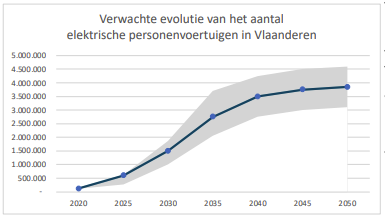
\includegraphics[scale=0.5]{img/Aantal_el_personenvoertuigen}
    \caption{\label{fig:Aantal_el_personenvoertuigen}Verwachte evolutie van het aantal
        elektrische personenvoertuigen in Vlaanderen \autocite{Verdoodt2022}.}
\end{figure}

\begin{figure}
    \centering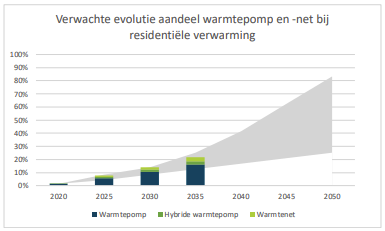
\includegraphics[scale=0.5]{img/Evolutie_Warmtepompen}
    \caption{\label{fig:Evolutie_Warmtepompen}Verwachte evolutie aandeel warmtepomp en -net bij
        residentiële verwarming \autocite{Verdoodt2022}.}
\end{figure}

\begin{figure}
    \centering\includegraphics[scale=0.5]{img/Evolutie_PV}
    \caption{\label{fig:Evolutie_PV}Verwachte evolutie PV (MWe) \autocite{Verdoodt2022}.}
\end{figure}

\begin{figure}
    \centering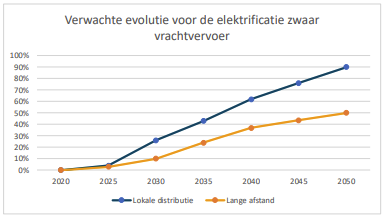
\includegraphics[scale=0.5]{img/El_Vrachtvervoer}
    \caption{\label{fig:El_Vrachtvervoer}Verwachte evolutie voor de elektrificatie zwaar
        vrachtvervoer \autocite{Verdoodt2022}.}
\end{figure}

Om al te hoge investeringen in de distributienetten te vermijden, wordt door Fluvius ingezet op maatregelen die de belasting van het elektriciteitsnet kunnen verminderen en spreiden. Een van die maatregelen is de invoering en verplichting van de digitale elektriciteitsmeter. Tegen juli 2029 moeten alle Belgische huishoudens een digitale meter hebben. Deze digitale meters kunnen via een dongle en een app 'slimmer' gemaakt worden, zodat gezinnen hun elektriciteitsverbruik in detail kunnen opvolgen en bijsturen. Dit zal dan meteen ook een besparing voor hen opleveren. Deze apps vereisen echter steeds een actieve opvolging van de gebruiker. Uit onderzoek is gebleken dat deze actieve bijsturing na verloop van tijd vermindert \autocite{Wemyss2019}. Een enquête van de \textcite{VREG2021} waarin 1.000 Vlaamse gezinnen en 1.500 bedrijven bevraagd werden over hun ervaring en gedrag op de energiemarkt toont zelfs aan dat van de 60\% van de gezinnen met een digitale meter, slechts 8\% hun energieverbruik effectief bijstuurt. Door de invoering van het capaciteitstarief, een andere maatregel waarmee de VREG het elektriciteitsnet hoopt te ontlasten, zal de bijsturing en vooral spreiding van het elektriciteitsverbruik nog belangrijker worden voor gezinnen. Sinds 1 januari 2023 wordt immers een deel van de nettarieven die een gezin via haar elektriciteitsfactuur betaalt ook berekend op het maximale elektriciteitsverbruik. Er wordt dus voortaan ook gekeken naar de maximale capaciteit die de distributienetbeheerders ter beschikking moeten stellen. Bedoeling van het capaciteitstarief is dat gezinnen hun stroomverbruik beter gaan spreiden. Als iedereen op hetzelfde moment veel stroom verbruikt, kan het net overbelast raken. Het gevolg is dat netbedrijven dan extra moeten investeren in zwaardere elektriciteitskabels om die hogere verbruikspieken op te vangen \autocite{Selleslagh2022}.

Daarom wordt binnen Fluvius de vraag gesteld hoe nieuwe technologieën en technieken een oplossing kunnen bieden om gezinnen te helpen bij het spreiden van hun elektriciteitsverbruik. Kunnen apps die het elektriciteitsverbuik monitoren slimmer gemaakt worden zodat ze geen tussenkomst van een gebruiker meer behoeven? Kan bijvoorbeeld artificiële intelligentie (AI) daarbij een oplossing bieden? Om dit na te gaan, zal tijdens dit onderzoek een app ontwikkeld worden die het elektriciteitsverbruik zal aansturen op basis van weersvoorspellingen en historische verbruiksdata.

\bigskip
\bigskip
\bigskip
\bigskip
\bigskip
\bigskip
\bigskip
\bigskip
\bigskip
\bigskip
\bigskip
\bigskip
\bigskip
\bigskip
\bigskip
\bigskip
\bigskip
\bigskip
\bigskip

\section{Literatuurstudie}%
\label{sec:literatuurstudie}

Met een digitale elektriciteitsmeter kunnen gezinnen hun elektriciteitsverbruik makkelijk opvolgen. Dat kan in de eerste plaats gratis via het online energieportaal \href{https://login.fluvius.be/klanten.onmicrosoft.com/b2c_1a_customer_signup_signin/oauth2/v2.0/authorize?client_id=91bb9a0a-f45d-491a-ae0b-43324fbc343a&scope=openid%20profile%20offline_access&redirect_uri=https%3A%2F%2Fmijn.fluvius.be%2Fredirect&client-request-id=90c12c72-7d7b-428b-98fc-5d7956e53a60&response_mode=fragment&response_type=code&x-client-SKU=msal.js.browser&x-client-VER=2.23.0&client_info=1&code_challenge=jz-1E8AwB15UEa352eC_5x6zDtAtwp3Je6jrFVdGKjk&code_challenge_method=S256&nonce=cee3d720-d931-4b13-b0b5-c473169ca6fd&state=eyJpZCI6IjRhM2I3M2NkLTgyZjgtNDFjOC05NzAyLTEwMTNjNjNkNjNhMyIsIm1ldGEiOnsiaW50ZXJhY3Rpb25UeXBlIjoicmVkaXJlY3QifX0%3D}{Mijn Fluvius}. Daarnaast bestaan er ook heel wat gratis of betalende online apps die op de gebruikerspoort van de digitale meter kunnen worden aangesloten om elektriciteitsverbruik op te volgen en de mogelijkheid bieden om andere toestellen aan te sturen. Een overzicht van deze toepassingen vindt men op de website \href{https://maakjemeterslim.be/}{www.maakjemeterslim.be}.

De digitale elektriciteitsmeter heeft twee gebruikerspoorten waar verschillende toestellen aan kunnen worden gekoppeld. Beide gebruikerspoorten zijn complementair en geschikt voor verschillende toepassingen. De P1-poort stuurt de elektriciteitsdata per seconde rechtstreeks uit. Via de ‘snelle’ S1-poort worden ruwe data aan een hoge frequentie ter beschikking gesteld. Beide poorten laten gedetailleerde verbruikersfeedback en sturing van huishoudapparaten toe. Op de gebruikerspoorten (P1 en/of S1) kan een energiebeheersysteem worden aangesloten \autocite{Depuydt2021}. Concreet gaat het om apps, slimme thermostaten of andere toestellen waarmee men elektriciteitsverbruik actief kan beheren. Zo’n toepassingen heten in het jargon ‘HEMS’ (Home Energy Management System) of ‘CEMS’ (Customer Energy Management System). De verbinding tussen het meettoestel en een app gebeurt in de meeste gevallen via een wifiverbinding of 4G.

De bestaande apps bieden allemaal de mogelijkheid om elektriciteitsverbruik in real time op te volgen. In elf gevallen kan dat naast een overzicht op de smartphone, tablet of computer ook via een afzonderlijk beeldscherm op de muur. Het meten van de energiekosten per huishoudtoestel behoort standaard tot verschillende apps, maar geldt ook vaak als een optie. De meeste apps sporen ook sluipverbruik op en bieden gepersonaliseerde tips voor energiebesparing. Sommige apps bieden tenslotte ook de mogelijkheid om het gemeten elektriciteitsverbruik naast weerdata te leggen en op die manier na te gaan hoeveel stroom men verbruikt bij bepaalde weersomstandigheden \autocite{Deman2021}. Het is duidelijk dat al deze apps slechts op een passieve het elektriciteitsverbruik van de gebruiker bijsturen. Het is de gebruiker zelf die op basis van de gevevens die de app hem toont actie kan ondernemen. En hoewel sommige bestaande apps efficiënter dan andere blijken \autocite{Mack2016} en \autocite{Wood2019}, leidt dit zoals reeds eerder werd vermeld, niet altijd tot de gewenste gedragsverandering \autocite{Wemyss2019}, \autocite{Mack2019} en  \autocite{VREG2021}.

Omdat het noodzakelijk is dat gezinnen en bedrijven bewuster en actiever met hun energieverbuik gaan omspringen, wordt binnen Fluvius en ook andere bedrijven gekeken naar nieuwe technologieën en technieken \autocite{Verdoodt2018}. Dit bracht mij op het idee om een app te gaan ontwikkelen die wel actief en dus automatisch het elektriciteitsverbruik kan gaan bijsturen. Omdat er reeds apps bestaan die weerdata gebruiken om het elektriciteitsverbruik onder bepaalde weersomstandigheden in kaart te brengen, lijkt het me zeker mogelijk om weerdata ook als aansturing te gaan gebruiken, samen met de historieken van het elektriciteitsverbruik om dan zo het toekomstig elektriciteitsverbruik en de elektriciteitsproductie te voorspellen \autocite{Guo2022}. Er zijn tal van bestaande gratis weer API's, zoals \href{https://openweathermap.org/api}{Open Weather Map} of \href{https://www.weatherapi.com/}{Weather API} die kunnen geïntegreerd worden in een app. Om de voorspellingen zo accuraat mogelijk te maken, zal gebruik gemaakt worden van het Extreme Gradient Boosting (XGBOOST) algoritme \autocite{Ledmaoui2023}, \autocite{Wang2022} en \autocite{BarreraAnimas2022}. De historische verbruiksdata, de productiedata van de omvormer van de zonnepanelen en de weerdata zullen als input gebruikt worden voor dit algoritme. De data van de digitale elekticiteitsmeter en de omvormer van de zonnepanelen wordt continue uitgelezen met een python script op een Raspberry Pi computer die via het wifi-netwerk verbonden is. Deze data wordt opgelsagen in een NoSQL-databank die speciaal voor time-series ontwikkeld is, nl. InfluxDB \autocite{Balis2017} en  \autocite{Struckov2019}. De app zal tenslotte ontwikkeld worden voor iOS en gebouwd worden met Xcode, SwiftUI en UIKit \autocite{Allardice} en \autocite{Firtman2022}.

De eerste slimme toestellen die via de app zullen worden beheerd zijn zonnepanelen en een warmtepomp \autocite{Uytterhoeven2019}. Door de afschaffing van de virtueel terugdraaiende teller voor eigenaars van zonnepanelen, waarbij de teller van de elektriciteitsmeter terugdraait wanneer meer elektriciteit wordt opgewekt dan verbruikt, kan het verlies van dit voordeel opgevangen door het verbruik van de warmtepomp te laten samenvallen met de productiemomenten van de zonnepanelen \autocite{Selleslagh2021}. Wanneer echter uit de weersverwachtingen blijkt dat er een aanzienlijke elektriciteitsproductie zal zijn, zal de app  mede op basis van historiek van het elektriciteitsverbruik automatisch ook andere toestellen, zoals de vaatwas of wasmachine gaan inschakelen. Om de sanitaire toestellen te kunnen gaan inschakelen, zal in de eerste plaats gekeken worden of deze toestellen van zichzelf reeds slim zijn. Meer concreet zal geverifieerd worden of ze over een Soft Real Time Operating System beschikken (Soft RTOS) en via het wifinetwerk kunnen communiceren met een app. Voor de sanitaire toestellen die niet slim zijn, zal gebruik gemaakt worden van slimme stopcontacten. Daarbij wordt er tussen het klassieke stopcontact en de stekker van het toestel een apparaat geplaatst, waardoor een toestel op een eenvoudige manier slim kan gemaakt worden \autocite{Jong2020}.

% Refereren naar de literatuur kan met:
% \autocite{BIBTEXKEY} -> (Auteur, jaartal)
% \textcite{BIBTEXKEY} -> Auteur (jaartal)
\newpage \pagebreak \cleardoublepage
\section{Methodologie}%
\label{sec:methodologie}

Het onderzoek zal aangevat worden met een studie van bestaande apps die kunnen verbonden worden met een digitale elektriciteitsmeter en waarmee elektricteitsverbruik kan opgevolgd en beheerd worden. Er bestaan heel wat gratis apps die elektriciteitsverbruik kunnen visualiseren en aansturen. Bedoeling is om een aantal van deze apps uitvoerig te gaan bestuderen. Wat zijn de functies die ze bieden. Hoe visualiseren deze apps het elektriciteitsverbruik en op welke manier kan het verbruik bijgestuurd worden. Door deze studie kan worden aangetoond dat de meeste van de apps om elektriciteitsverbruik te beheren louter passief werken en steeds een actie van de gebruiker vereisen.

In het tweede deel van het onderzoek zal een app ontwikkeld worden die met behulp van artificiële intelligentie historische verbruiksdata en weersvoorspellingen zal gebruiken om het elektriciteitsverbruik automatisch aan te sturen en te beheren. Vooreerst zal de data van de digitale elektriciteitsmeter worden uitgelezen met behulp van een Raspberry Pi 2GB. De uitgelezen data zal worden opgeslagen in een Azure databank. Wanneer voldoende verbruiksdata verzameld is, zal artificiële intelligentie gebruikt worden om toekomstig elektriciteitsverbruik te voorspellen. Daarvoor zal in eerste instantie gekeken worden naar een bestaand AI platform zoals Azure AI van Microsoft. Om de voorspelling nog acurater te kunnen maken, zal de historische verbruiksdata gecombineerd worden met weersvoorspellingen van een open source weer API. De voorspellingen zullen vervolgens gebruikt worden om slimme of slim gemaakte toestellen automatisch te gaan in- of uitschakelen. Om dit alles inzichtelijk te maken voor de gebruiker zal een mobiele applicatie in IOS ontwikkeld worden. Via deze mobiele applicatie zal de gebruiker ook de mogelijkheid hebben om handmatig bij te sturen indien hij of zij dit wenst.

Nadat de app ontwikkeld is, zal een selectie worden gemaakt van welke elektrische toestellen de app zal aansturen. Er zal nagegaan worden met welke toestellen het meeste elektriciteit bespaard kan worden door ze met weersvoorspellingen aan te sturen. Verder zal ook bepaald worden op welke manier de gekozen toestellen slim kunnen gemaakt worden. Zijn de toestellen reeds slim van zichzelf, zoals bijvoorbeeld sommige zonnepanelen dat zijn, of moeten de toestellen slim gemaakt worden? Een optie daarbij is het gebruik van slimme stopcontacten. Daarbij kan er tussen het klassieke stopcontact en de stekker van het toestel een apparaat geplaatst worden, waardoor een klassiek stopcontact zonder ingrijpende werken slim kan gemaakt worden.

%Om na te gaan of de app een elektriciteitsbesparing oplevert, zullen een aantal testgebruiker de app gedurende een maand testen. Om de werking van de app te kunnen testen zullen vijf testgebruikers geselecteerd worden. Zij zullen de app gedurende een maand gebruiken. In de eerste plaats zal de testgebruikers gevraagd worden om elke dag na te gaan of en wanneer de verbonden slimme toestellen door de app aangestuurd werden. In de app zal namelijk steeds een overzicht van de in- en afschakelmomenten van de verschillende toestellen beschikbaar zijn. Daarnaast zullen de testgebruikers ook gevraagd worden om een manuele bijsturing te noteren en kort de reden hiervan te vermelden. Telkens wanneer de app een verbonden toestel niet correct in- of uitschakelt, kan de gebruiker tussenkomen en het desbtreffende toestel zelf in- of uitschakelen. Na afloop van deze onderzoeksfase zullen vijf testgebruikers, waaronder de onderzoeker zelf, de app gedurende een maand getest hebben.

Na de testperiode zal worden geverifieerd in welke mate de app de ermee verbonden apparaten correct heeft in- en uitgeschakeld. Meer concreet zal worden nagegaan hoe vaak de door de app aangestuurde toestellen correct werden in- of uitgeschakeld. Daarvoor zullen de door de app geregistreerde gegevens vergeleken worden met de door de testgebruikers genoteerde manuele tussenkomsten. Ook zal de testgebruikers een vragenlijst worden voorgelegd, waarin naar hun ervaringen met het gebruik van de app gepeild wordt. Zo zal er gevraagd worden of de app op de juiste momenten de ermee verbonden toestellen in- en uitschakelde. Er zal een verslag worden opgemaakt waarin per testgebruiker en per toestel de manuele bijsturingen in kaart worden gebracht. Hieraan zullen ook de antwoorden op de vragenlijst worden toegevoegd, zodat per testgebruiker een conclusie kan getrokken worden.

\section{Verwachte resultaten}%
\label{sec:verwachte-resultaten}

De verwachting is dat na afloop van dit onderzoek de zelfconsumptie van de testdeelnemers verhoogd is en het elektriciteitsverbruik meer gespreid wordt. Om hieruit ook werkelijk een financieel voordeel te halen, zal de minstens 50\% zelfverbruik moeten behaald worden \autocite{Selleslagh2021}. Als naast de warmtepomp ook een wasmachine, vaatwasmachine en een elektrisch voertuig kunnen worden aangesloten op de ontwikkelde app, zal dit percentage zeker behaald kunnen worden. 

Omdat ook piekverbruiken moeten vermeden worden omwille van het capaciteitstarief, zal de app enkel toestellen inschakelen indien de elektriciteit die door de zonnepanelen gegenereerd wordt toereikend is om aan het gecombineerde verbruik te voldoen. Op basis van de weersverwachtingen zal de app gaan inschatten of de productie voldoende lang kan gegarandeerd worden. Zo zullen meerdere toestellen tegelijkertijd kunnen worden ingeschakeld zonder een verbruikspiek te veroorzaken. Omgekeerd zal de app er ook voor zorgen dat op dagelijkse piekmomenten sommige toestellen worden uitgeschakeld, indien er onvoldoende elektriciteit wordt opgewekt door de zonnepanelen. Zo zal de warmtepomp uitgeschakeld worden op het moment dat al veel andere apparaten aan het werk zijn. Verwacht wordt dat de app de piekverbruiken zo automatisch tot een minimum zal herleiden, waardoor de nettarieven en dus de elektriciteitsfactuur voor gezinnen kan verlaagd worden.
\autocite{Balakumar2023} \autocite{Gozuoglu2024}  \autocite{Tziolis2024}  \autocite{Guerra2024}  \autocite{Bozlak2024}  \autocite{Kim2023} \autocite{Hoseinpour2024}  \autocite{Volta2023} \autocite{Konsman2023} \autocite{Fluvius2023}

%\section{Discussie, conclusie}%
%\label{sec:discussie-conclusie}

\bigskip
\bigskip
\bigskip
\bigskip
\bigskip
\bigskip
\bigskip
\bigskip
\bigskip
\bigskip
\bigskip
\bigskip
\bigskip
\bigskip
\bigskip
\bigskip
\bigskip
\bigskip
\bigskip


%------------------------------------------------------------------------------
% Referentielijst
%------------------------------------------------------------------------------
% bibliografie.bib voorkomen. Gebruik JabRef om je bibliografie bij te
% houden.

\printbibliography[heading=bibintoc]

\end{document}

%%---------- Andere bijlagen --------------------------------------------------
% TODO: Voeg hier eventuele andere bijlagen toe. Bv. als je deze BP voor de
% tweede keer indient, een overzicht van de verbeteringen t.o.v. het origineel.
%\input{...}

%%---------- Backmatter, referentielijst ---------------------------------------

\backmatter{}

%\setlength\bibitemsep{2pt} %% Add Some space between the bibliograpy entries
\printbibliography[heading=bibintoc]

\end{document}
